%--------------------------------------------------------------------
% Эта преамбула с комментариями для написания лабораторных работ по
% физике. В еe основе информация из книги С. М. Львовского "Набор и
% верстка в пакете Latex", а также материалы по курсу "Документы и
% презентации в Latex" от ВШЭ https://www.coursera.org/learn/latex. Ну
% и мой опыт (1 год и 16 лабораторных работ + 2 Вопроса по выбору)
% Автор - Баринов Леонид
% Дата - 06.08.2019
%--------------------------------------------------------------------
%--------------------------------------------------------------------
% Для начала необходимо определиться с типом документа. Оптимальный
% (на мой взгляд) вариант - article. Также существуют типы book,
% report, proc и другие. Также в необязательном аргументе можно
% указать тип страницы и размер шрифта. Стандарт по умолчанию - А4 и
% 12 (иногда 10) шрифт. Необязательный аргумент шрифта может принимать
% только 3 параметра - 10, 11, 12 (pt).

\documentclass[a4paper, 12pt]{article}

%--------------------------------------------------------------------
% Чтобы использовать другие размеры шрифта используется пакет
% extsizes. Он позволяет указывать в \documentclass такие размеры - 8,
% 9, 10, 11, 12, 14, 17, 20 (pt). При указании других размеров могут
% возникать различные проблемы.

\usepackage{extsizes}

%--------------------------------------------------------------------
% Необходимо определиться с кодировкой документа. Идеального варианта
% для русского языка не существует - каждый чем-то немного плох. Для
% особо интересующихся - Приложение И в 5 издании книги Львовского. Я
% воспользовался вариантом, предлагаемым на курсе по Latex от ВШЭ.

\usepackage[T2A]{fontenc}
\usepackage[utf8]{inputenc}

%--------------------------------------------------------------------
% Для соблюдения типографских традиций (оказывается такие существуют)
% различных стран создан пакет babel. Самое заметное его действие -
% latex научиться переносить слова того языка, который вы укажите.
% Можно указать несколько языков через запятую. Основной язык
% документа указывается последним.

\usepackage[english,russian]{babel}

%--------------------------------------------------------------------
% Перейдем к заданию полей документа. Есть несколько способов, но
% самый простой из них - это воспользоваться пакетом geometry, который
% позволяет определить все поля документа (начиная с краев листа, что
% важно, так как некоторые другие способы позволяют это сделать только
% косвенно)

\usepackage{geometry}
\geometry{top=25mm}
\geometry{bottom=35mm}
\geometry{left=35mm}
\geometry{right=20mm}

%--------------------------------------------------------------------
% От полей логично перейти к колонтитулам. Тут нам поможет пакет
% fancyhdr. Для него существует 6 колонтитулов - верхний, левый;
% верхний, по центру; верхний, правый и такие же нижние. По умолчанию
% номер страницы находится снизу по центру, а также существует
% линейка, очерчивающие верхний колонтитул. Мне показалось интересным
% сделать колонтитулы схожие с колонтитулами в лабнике. 

\usepackage{fancyhdr}
\pagestyle{fancy}
\renewcommand{\sectionmark}[1]{\markboth{#1}{}} 
% \renewcommand{\headrulewidth}{0mm} % Если необходимо убрать линейку,
% или изменить ее длину
% \lfoot{} % Нижний левый
% \rfoot{} % Нижний правый
% \rhead{} % Верхний правый
% \chead{} % Верхний в центре
\lhead{\thepage} % Номер страницы в левом верхнем углу
\cfoot{} % Оставить нижний колонтитул без цифры

%--------------------------------------------------------------------
% Самое время научиться работать с формулами. А точнее добавить пакеты
% от Американского математического общества, которые позволять
% пользоваться большим количеством математических символов.

\usepackage{amsmath,amsfonts,amssymb,amsthm,mathtools}

%--------------------------------------------------------------------
% Также очень хочется пользоваться русскими буквами в формулах, для
% этого подключаем пакет mathtext, который добавляет окружение
% \text{}. Внутри него можно писать русские буквы в математическом
% режиме.

\usepackage{mathtext}

%--------------------------------------------------------------------
% Большим преимуществом вашего pdf документа будет возможность поиска
% в нем по словам или буквами. (Например, в Ивановнике это
% невозможно)

\usepackage{cmap}

%--------------------------------------------------------------------
% Куда же в физике без картинок и графиков? Давайте исправим
% эту недоработку

\usepackage{graphicx}
\graphicspath{images/} % Необходимо, если рисунки
% находятся в другой папке

%--------------------------------------------------------------------
% graphicx не позволяет вставлять обтекаемые рисунки, но на
% практике они очень нужны. Для этого существует пакет wrapfig

\usepackage{wrapfig}

%--------------------------------------------------------------------
% latex вставляет рисунки по определенному алгоритму. Его,
% конечно, можно менять, но это не настолько просто. Как
% правило, хочется, чтобы картинка располагалась там, где мы это
% указали в коде. Для этого существует несколько пакетов, один из
% них floatrow. Он позволяет для окружения figure указывать
% необязательный аргумент - H (именно большое h), что на latex'овском
% языке означает: вставить картинку здесь и только здесь. (даже если
% облик документа несколько пострадает)

\usepackage{floatrow}

%--------------------------------------------------------------------
% По правилам оформления рисунок всегда должен быть подписан. Для
% этого существует команда \caption{}. Но обычные настройки caption
% меня не совсем устроили. Хотелось сделать подпись меньше
% основного шрифта, а также слово Рис жирным и использовать
% разделитель точку, а не двоеточие. В этом помогает пакет,
% который называется caption (совпадение?)

\usepackage[margin=10pt,font=small,labelfont=bf,labelsep=period]{caption}

%--------------------------------------------------------------------
% Последним важным пунктом остались таблицы. Ведь куда-то нужно
% заносить результаты измерений. На данный момент во время выполнения
% лабораторных работ я заношу результаты в таблицу excel, а потом с
% помощью сайта www.tablesgenerator.com превращаю в таблицу latex и
% дооформляю.

\usepackage{array,tabularx,tabulary,booktabs}

%--------------------------------------------------------------------
% После excel есть ощущения, что везде объединить колонки или строки
% легко. В latex не совсем так. Помогают пакеты multirow, multicol. 

\usepackage{multirow}
\usepackage{multicol}

%--------------------------------------------------------------------
% Иногда могут потребоваться длинные таблицы на несколько страниц.
% Обычные таблицы latex воспринимает как одну букву. И
% становиться понятно, почему возникают проблемы при переносе
% обычной таблицы. (Ведь нельзя же перенести одну букву!). Поэтому
% вместо обычной таблицы нужна длинная таблица.

\usepackage{longtable}

%--------------------------------------------------------------------
% Часто в таблице хочется сделать перенос текста или формулы. Просто
% так это сделать не получиться из-за синтаксиса tabular. Для этого
% каждый раз необходимо создавать новое окружение tabular, что
% утомительно. Поэтому можно ввести команду \specialcell
% (назвать можно по-любому)
    
\newcommand{\specialcell}[2][c]{%
	\begin{tabular}[#1]{@{}c{}}#2\end{tabular}}

%--------------------------------------------------------------------
% Когда в таблице много колонок и строк, кажется, что они находятся
% слишком близко к друг другу. Можно переопределить
% несколько параметров, чтобы выглядело лучше. Это можно сделать либо
% в преамбуле, либо непосредственно в документе. Первое
% переопределение отвечает за интервал между строками, второе за
% интервал между колонками

% \renewcommand{\arraystretch}{1.8} 
% \renewcommand{\tabcolsep}{1cm} 

%--------------------------------------------------------------------
% В русской типографской традиции принято начинать каждый новый абзац
% с красной строки. Даже первый после заголовка (или подзаголовка).
% Чтобы каждый раз не ставить красную строку вручную существует пакет
% indentfirst

\usepackage{indentfirst}

%--------------------------------------------------------------------
% Некоторые модификаторы начертания

\usepackage{soul}
\usepackage{soulutf8}
 
\begin{document}
\thispagestyle{empty}
\begin{center}
    \textit{Федеральное государственное автономное образовательное\\ учреждение высшего образования }

    \vspace{0.5ex}

        \textbf{«Московский физико-технический институт\\ (национальный исследовательский университет)»}
\end{center}

\vspace{10ex}

\begin{center}
    \vspace{13ex}

    \so{\textbf{Лабораторная работа №_._._}}

    \vspace{1ex}

    по курсу общей физики

    на тему:

    \textbf{\textit{<<>>}}

    \vspace{30ex}

    \begin{flushright}
        \noindent
        \textit{Работу выполнил:}\\  
        \textit{Баринов Леонид \\(группа Б02-827)}
    \end{flushright}
    \vfill
    Долгопрудный \\2019
\newpage
\setcounter{page}{1}
\fancyhead[R]{\nouppercase{\leftmark}}	
\end{center}

\section{Аннотация}
В работе будет проведено изучение
спектрального состава периодических
электрических сигналов.

\section{Теоретические сведения}
Сколь угодно сложный электрический
сигнал $ U(t) $ может быть разложен на
более простые сигналы. В радиотехнике
широко используется разложение входного
сигнала $ U(t) $ на совокупность
\textit{гармонических сигналов}
различных частот $\omega$. Функция
$F(\omega)$, описывающая зависимость
амплитуд отдельных гармоник от частоты,
называется \textit{амплитудной
спектральной характеристикой сигнала} $
U(t) $. Представление сложного
периодического сигнала в виде суммы
дискретных гармонических сигналов в
математике называется разложением в ряд
Фурье (или \textit{прямым
преобразованием Фурье}). Зная
спектральный состав  $F(\omega)$
периодической последовательности
некоторого импульса $ U(t) $, мы можем
осуществить \textit{ обратное
преобразование Фурье}: сложив отдельные
гармоники с различными амплитудами и
фазами, получить необходимую
последовательность импульсов. Степень
совпадения полученного сигнала с $ U(t)
$ определяется количеством
синтезированных гармоник: чем их больше,
тем лучше совпадение. Однако, если в
развертке спектра нет острых уступов,
даже небольшое количество гармоник
обеспечивает достаточно точное
совпадение теоретической и наблюдаемой
картин спектра.


Введем формальное определение понятия
<<спектр>>. Для этого рассмотрим функцию вида:
\begin{equation}
f(t)=\sum_{n=1}^{N} A_{n} \cos \left(\omega_{n} t-\alpha_{n}\right),
\end{equation}
где $A_{n}$, $\omega_{n}$, $\alpha_{n}$ - постоянные величины. Спектром функции $f(t)$ называется набор
$(\omega_{i}, A_{i})$. Данное определение применимо и в случае $N \rightarrow \infty$.

Рассмотрим подробнее два вида входных сигналов: периодический и непериодический.

\subsection*{Фурье-спектр периодических сигналов}

Пусть заданная функция $f(t)$
периодически повторяется с частотой
$\Omega_{1} = \frac{2\pi}{T}$. Её
разложение в ряд Фурье имеет вид
\begin{equation}
\begin{aligned} 
f(t) &= \frac{a_{0}}{2}+\sum_{n=1}^{\infty}\left[ a_{n} \cos \left(n\Omega_{1} t\right) + b_{n} \sin \left(n \Omega_{1} t\right)\right] \\ f(t) &= \frac{A_{0}}{2}+\sum_{n=1}^{\infty} A_{n} \cos \left(n \Omega_{1} t-\psi_{n}\right)
\end{aligned}
\end{equation}

Здесь $a_{0}/2 =A_{0}/2$ — среднее значение функции $ f(t) $; $ a_{n} $ и $ b_{n} $ — амплитуды косинусных и синусных членов разложения, которые определяются соотношениями 

\begin{equation}
\begin{aligned} a_{n} &=\frac{2}{T}
\int\limits_{t_{1}}^{t_{1}+T} f(t) \cos \left(n
\Omega_{1} t\right) d t \\ b_{n}
&=\frac{2}{T} \int\limits_{t_{1}}^{t_{1}+T}
f(t) \sin \left(n \Omega_{1} t\right) d
t \end{aligned}
\end{equation}
Точка начала интегрирования выбрается произвольно.

Если сигнал чётен относительно $  t = 0 $, в тригонометрической записи остаются только косинусные члены. Для нечётной относительно $ t = 0  $ функции, наоборот, в нуль обращаются коэффициенты $ a_{n} $, и ряд состоит только из синусных членов.

Амплитуда $ A_{n} $и фаза $\psi_{n}$ $n-$й гармоники естественным образом выражаются через $a_{n}$ и $b_{n}$:

\begin{equation}
A_{n}=\sqrt{a_{n}^{2}+b_{n}^{2}} ; \quad \psi_{n}=\operatorname{arctg} \frac{b_{n}}{a_{n}}.
\end{equation}

Как мы видим, спектр любой периодической функции состоит из набора гармонических колебаний с дискретными частотами и некой постоянной составляющей, которую можно рассматривать как колебание с нулевой частотой.

Приведем основные факты о периодических сигналах, исследуемых в данной работе.


\subsection*{Исследование спектра периодической последовательности прямоугольных импульсов}

Периодическая последовательность прямоугольных импульсов с амплитудой $ V(t) $, длительностью $\tau$, частотой повторения $ f_{повт} = 1/T $, где $ T $ — период повторения импульсов.

\begin{figure}[H]
    \floatsetup{heightadjust=object,valign=c}
    \begin{floatrow}
        \ffigbox{\captionsetup{justification=centering}\caption{Периодическая
        последовательность прямоугольных
импульсов}}%
        {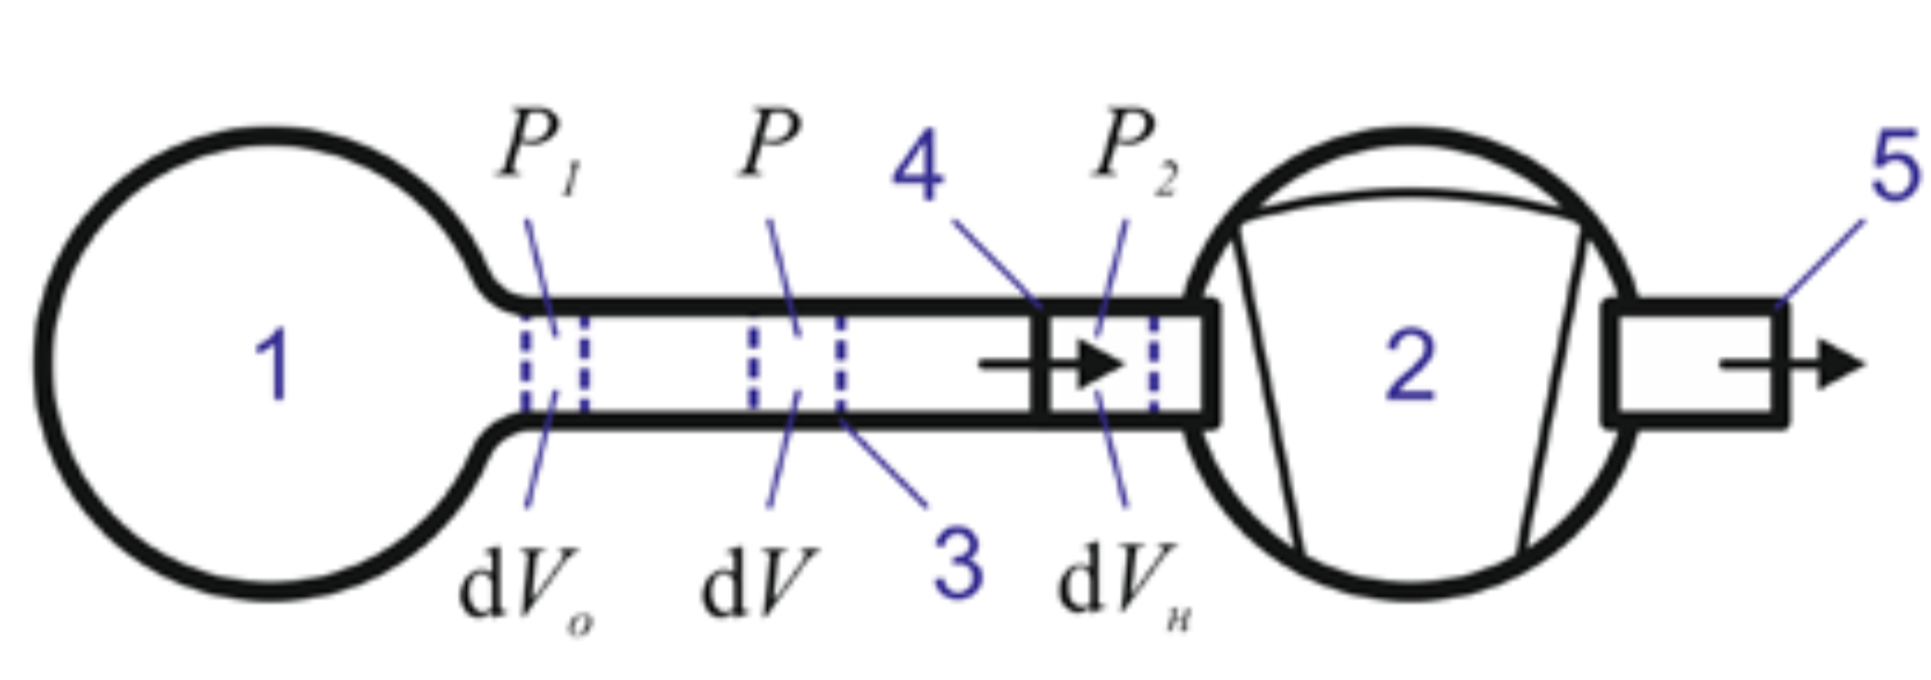
\includegraphics[width
        =\linewidth]{1}}
        \ffigbox{\captionsetup{justification=centering}\caption{Спектр
        периодической последовательности
прямоугольных импульсов}}%
        {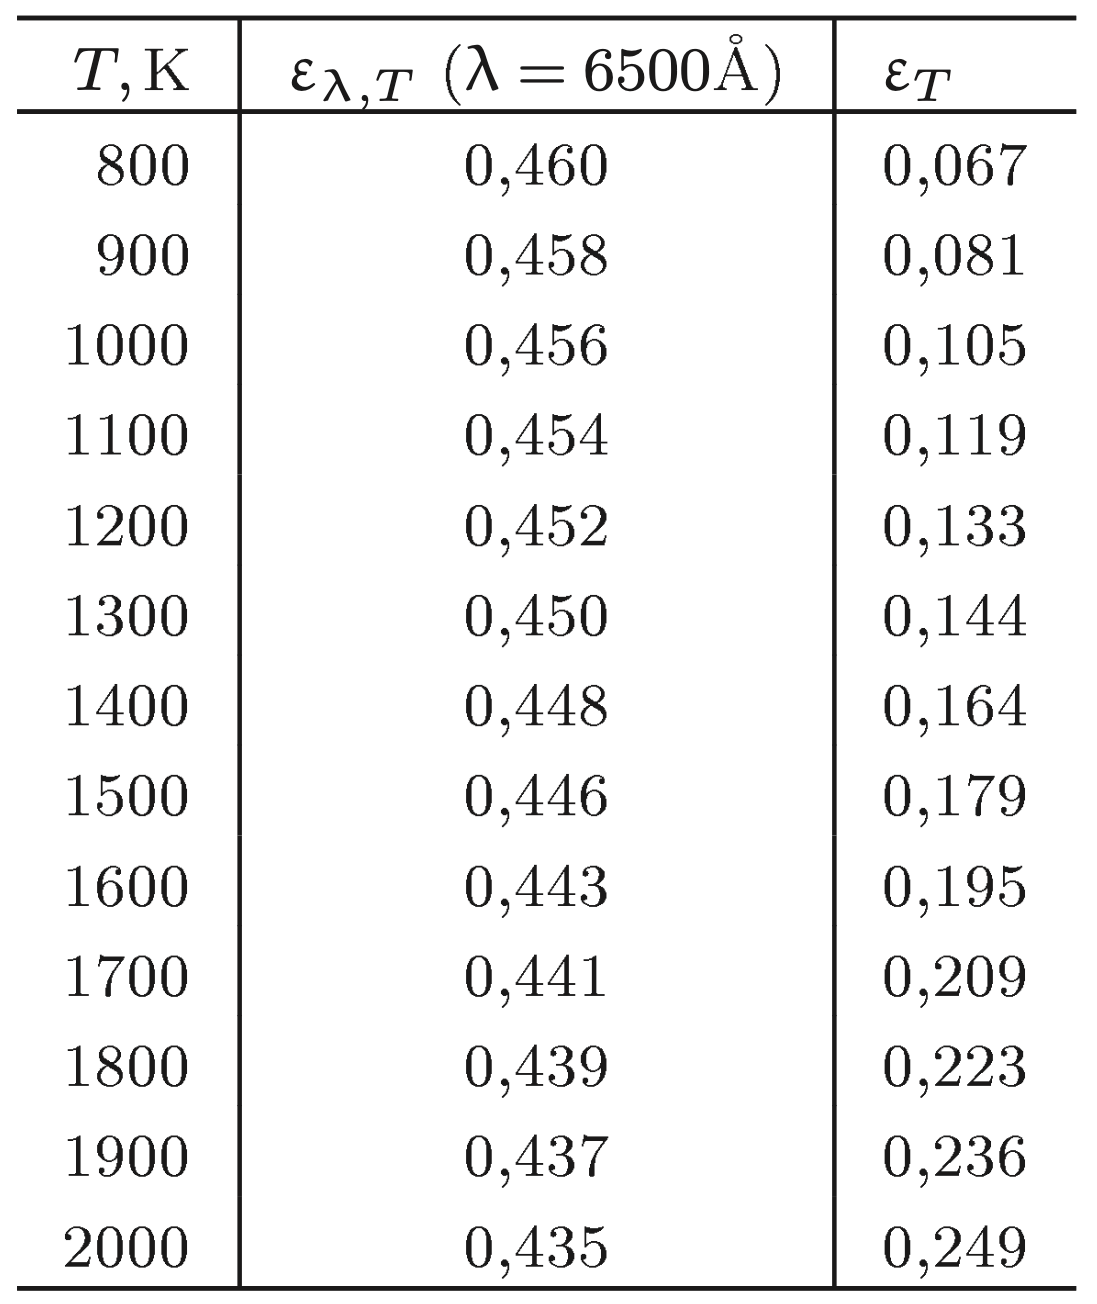
\includegraphics[width=\linewidth]{2}}        
    \end{floatrow}
\end{figure}

На рис. 2 изображен случай, когда $T$
кратно $\tau$. Назовем шириной спектра
$\Delta \omega$ (или $\Delta \nu =
\Delta \omega/2\pi$) расстояние от
главного максимума $(\omega = 0)$ до
первого нуля огибающей, возникающего при
$n = 2\pi/\tau \Omega_1$. При этом 
\begin{equation}
    \Delta \omega \tau \approx 2\pi \
    \text{или} \ \Delta \nu \Delta t
    \approx 1
\end{equation}
Полученной соотношение взаимной связи
интервалов $\Delta \nu$ и $\Delta t$
является частным случаем соотношения
неопределенности в квантовой механике.

\begin{equation}
\begin{gathered}
\langle V\rangle = \frac{a_{0}}{2} = V_{0} \frac{\tau}{T} \\
\hat{f}(\omega) = \frac{1}{\sqrt{2
\pi}} \int\limits_{-\infty}^{\infty} f(x) e^{-i
x \omega} d x \\
a_{n}=2 V_{0} \frac{\tau}{T} \frac{\sin \left(n \Omega_{1} \tau / 2\right)}{n \Omega_{1} \tau / 2} \sim \frac{\sin x}{x}
\end{gathered}
\end{equation}


\subsection*{Исследование спектра периодической последовательности цугов гармонических колебаний }


Периодическая последовательность цугов гармонического колебания $ V(t) = V_{0}\cos(\omega_{0}t) $ с длительностью цуга $\tau$ и периодом повторения $T$.




\begin{figure}[H]
    \floatsetup{heightadjust=object,valign=c}
    \begin{floatrow}
        \ffigbox{\captionsetup{justification=centering}\caption{Периодическая
        последовательность цугов}}%
        {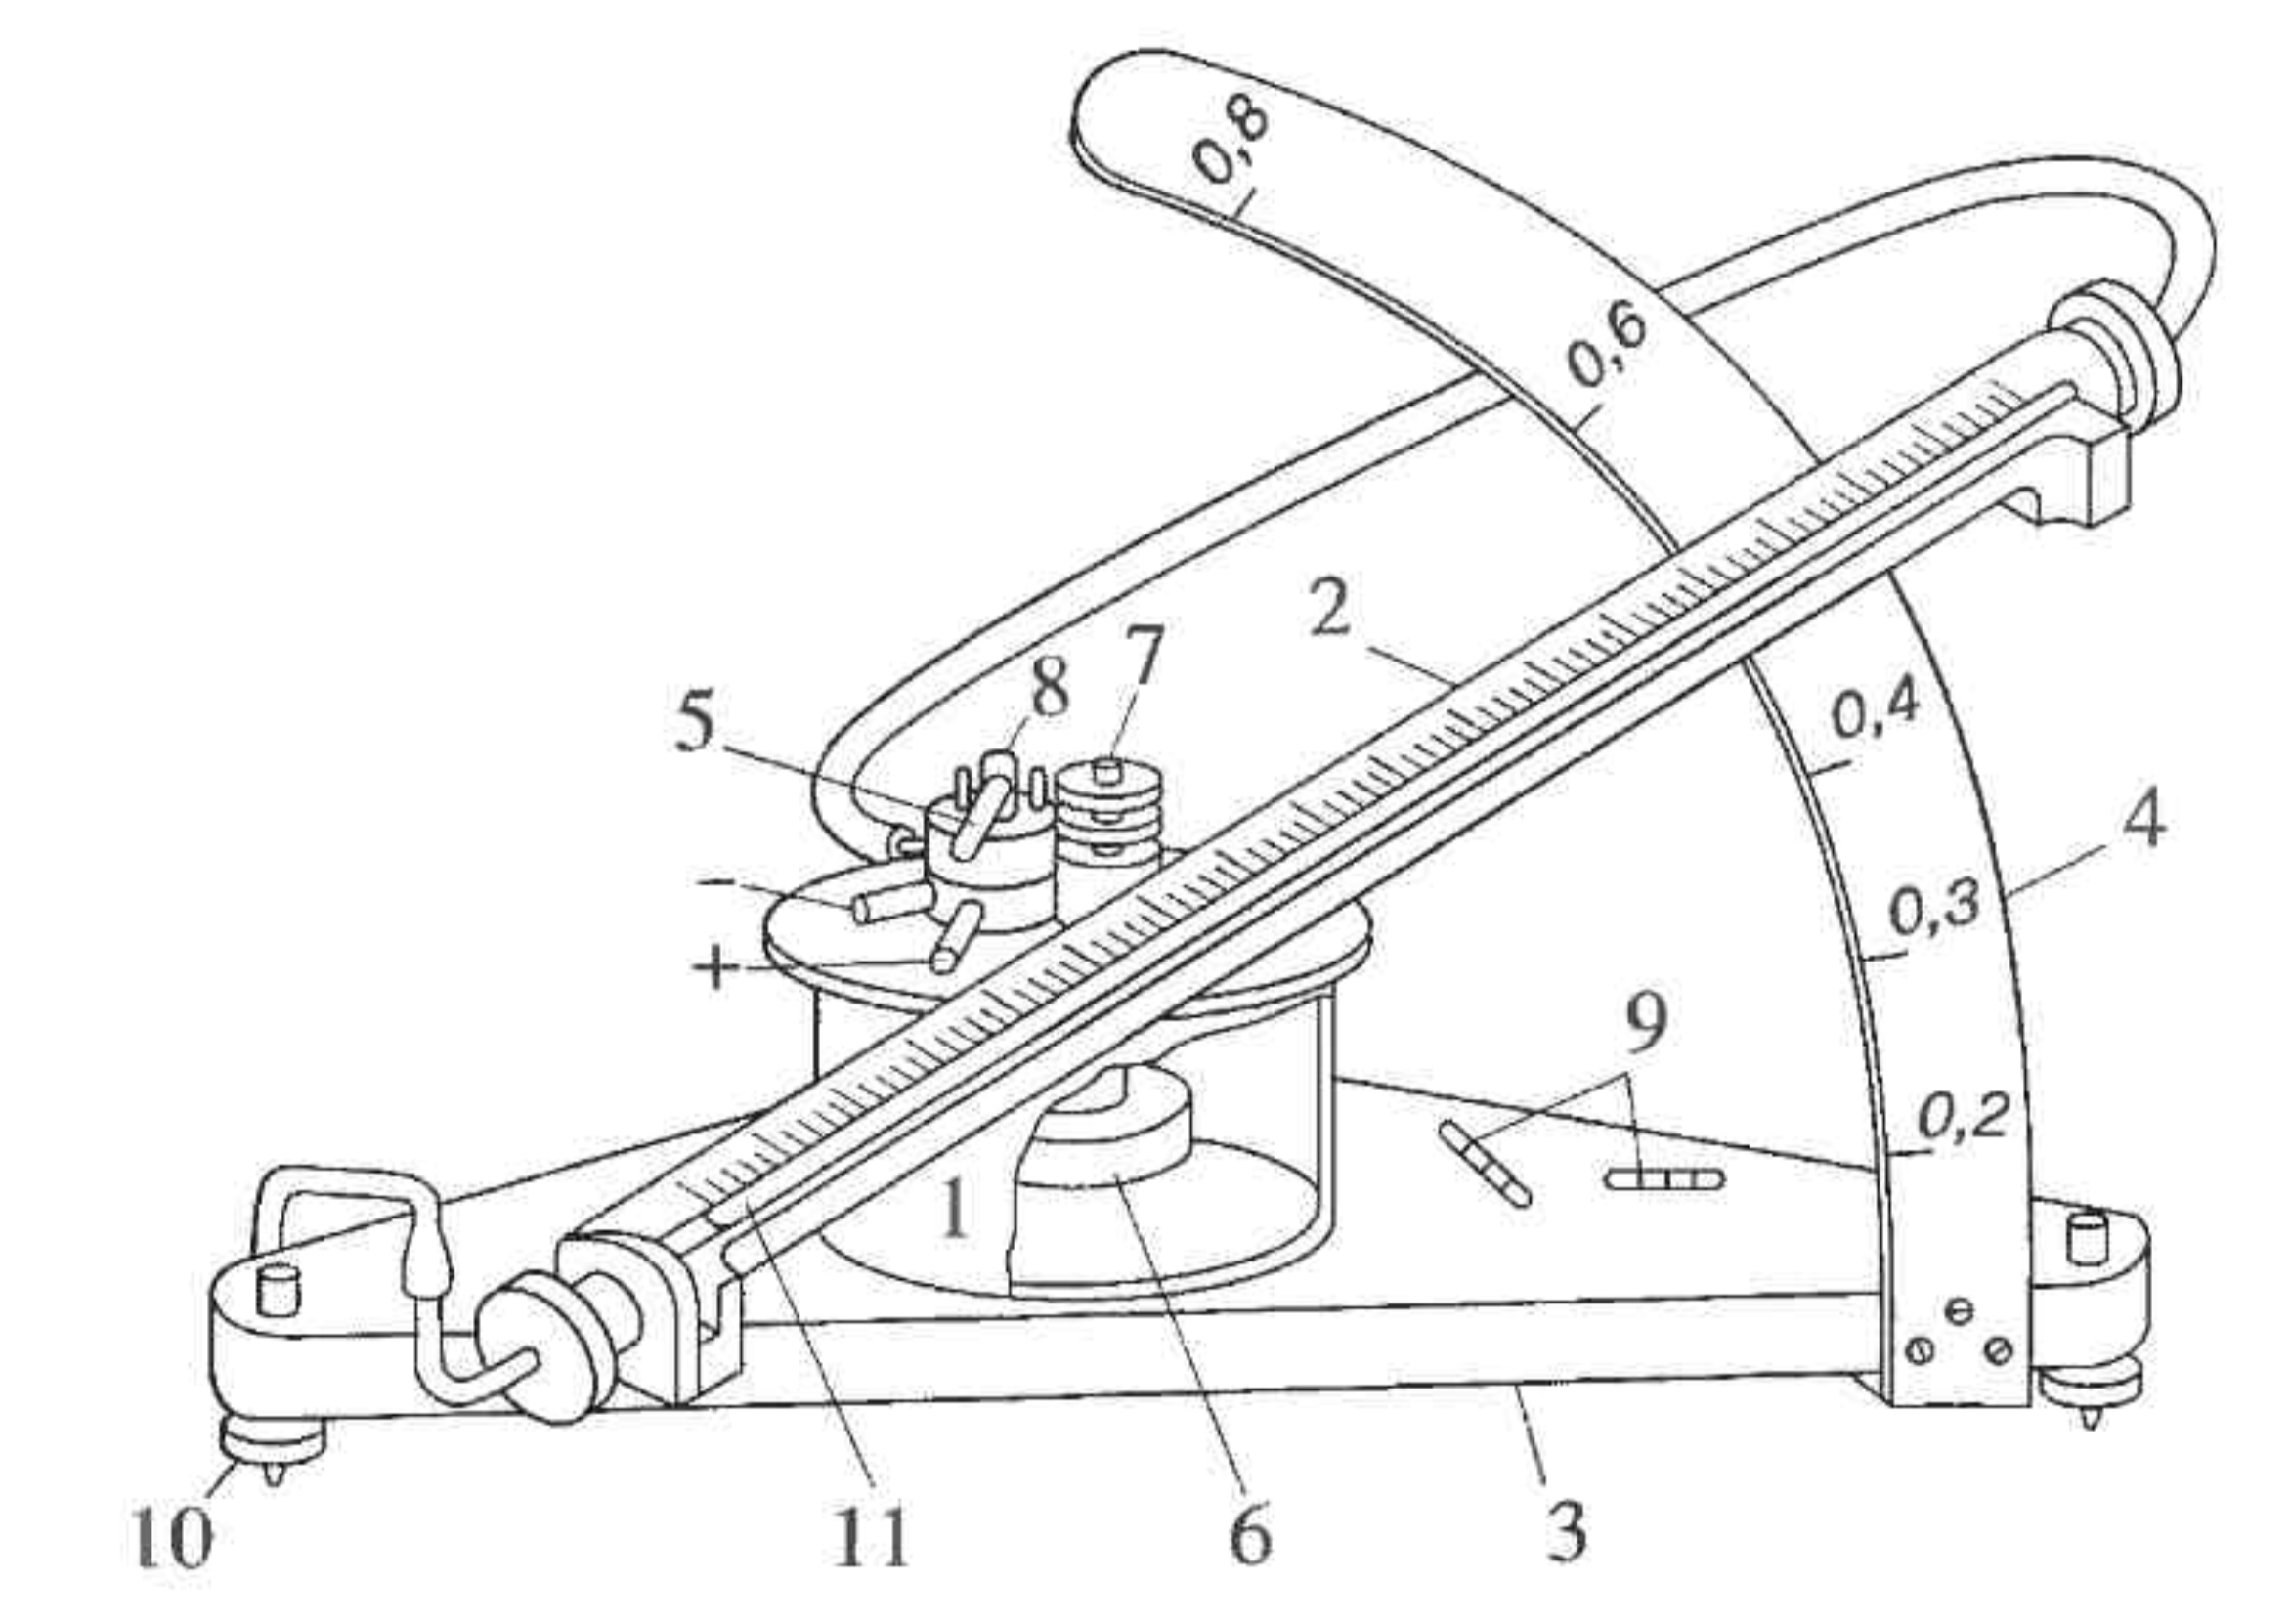
\includegraphics[width
        =0.9\linewidth]{3}}
        \ffigbox{\captionsetup{justification=centering}\caption{Спектр
        периодической последовательности
цугов}}%
        {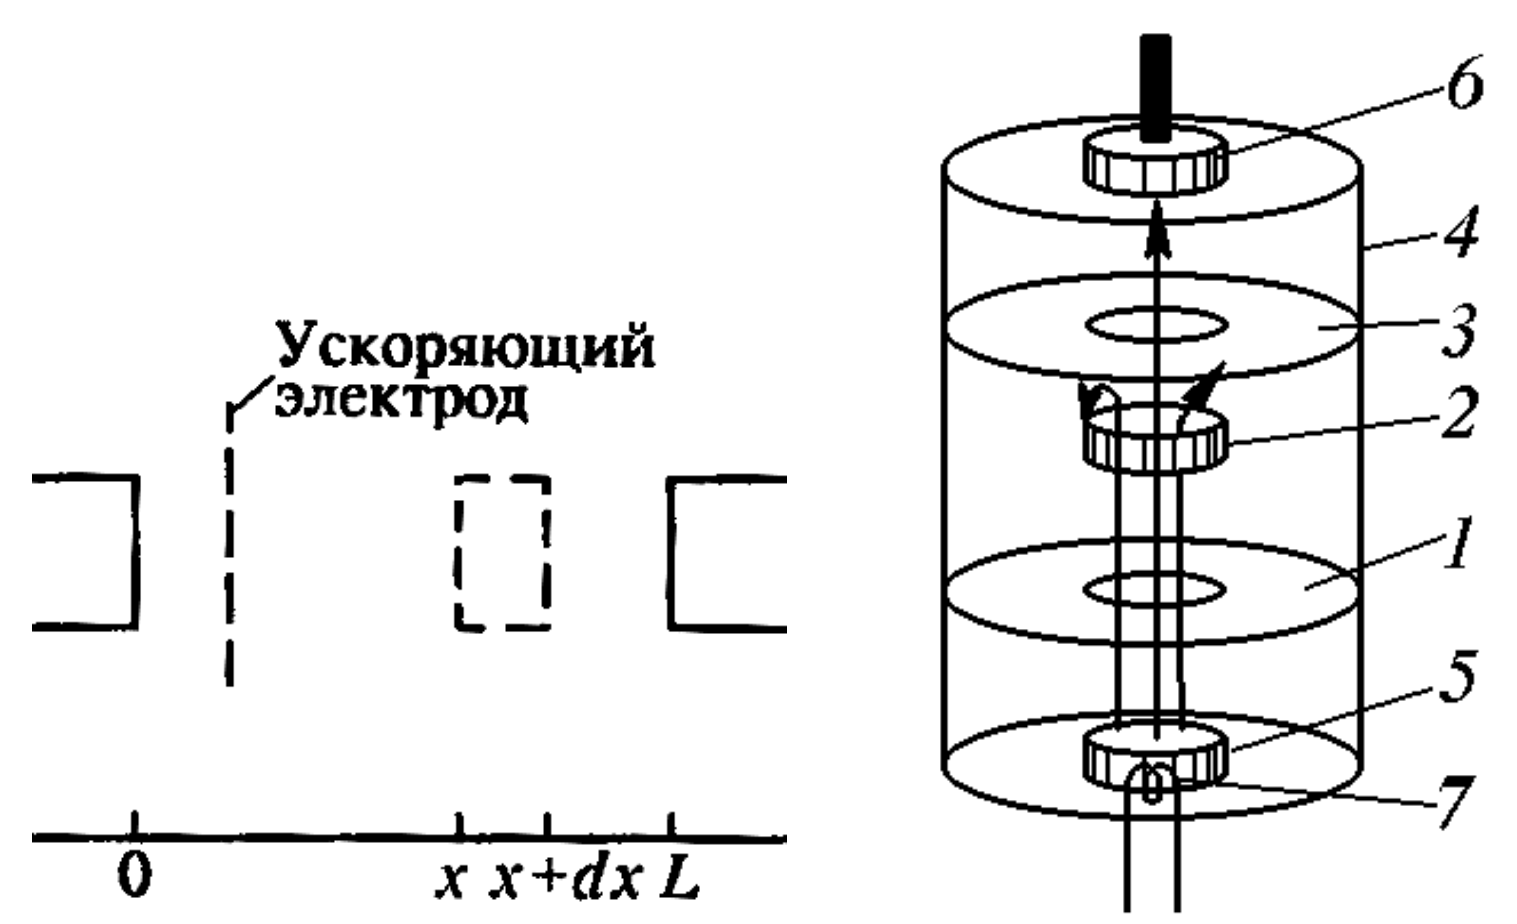
\includegraphics[width=0.9\linewidth]{4}}        
    \end{floatrow}
\end{figure}

\begin{equation}
A_{n} =  V_{0}
\frac{\tau}{T}\left(\frac{\sin
\left[\left(\omega_{0}-n
\Omega_{1}\right)
\frac{\tau}{2}\right]}{\left(\omega_{0}-n
\Omega_{1}\right)
\frac{\tau}{2}}+\frac{\sin
\left[\left(\omega_{0}+n
\Omega_{1}\right)
\frac{\tau}{2}\right]}{\left(\omega_{0}+n
\Omega_{1}\right) \frac{\tau}{2}}\right)
\end{equation}

\subsection*{Исследование спектра гармонических сигналов, модулированных по амплитуде}

Рассмотрим колебания высокой частоты,
амплитуда которых медленно меняется по
гармоническому закону с частотой $\Omega
\left(\Omega \ll
\omega_{0}\right)$:\newline
$f(t)=A_{0}[1+m \cos (\Omega t)] \cos
(\omega t)$.

Коэффициент $m$ называют глубиной модуляции. При $m < 1$ амплитуда колебаний меняется от минимальной $A_{\min }=A_{0}(1-m)$ до максимальной $A_{\max }=A_{0}(1+m)$. Глубина модуляции может быть представлена в виде 
\begin{equation}
m=\frac{A_{\max }-A_{\min }}{A_{\max }+A_{\min }}
\end{equation} 

\begin{figure}[H]
    \floatsetup{heightadjust=object,valign=c}
    \begin{floatrow}
 \ffigbox{\captionsetup{justification=centering}\caption{Гармонические
        колебания, модулированные по
амплитуде}}%
{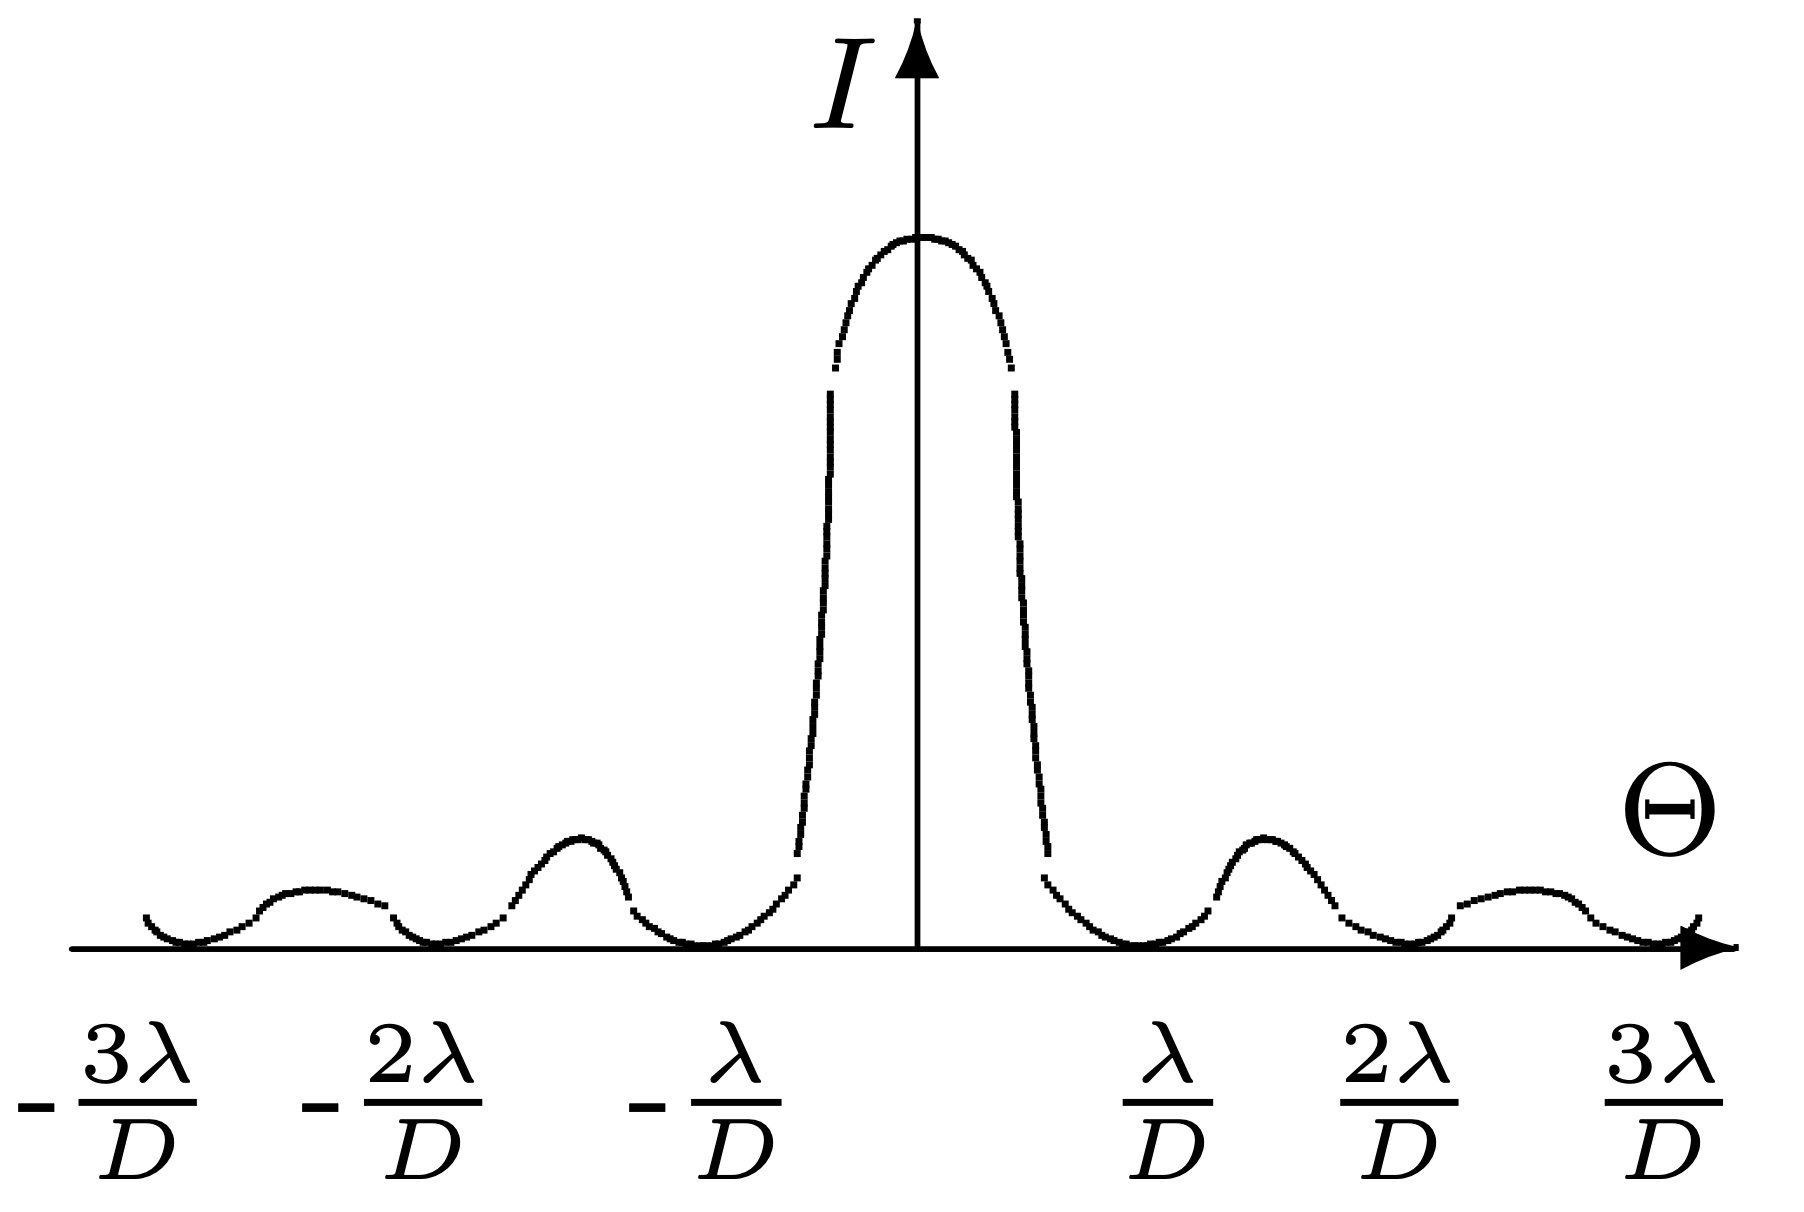
\includegraphics[width=\linewidth]{5}}
        \ffigbox{\captionsetup{justification=centering}\caption{Спектр
        синусоидальных колебаний,
модулированных по амплитуде}}%
        {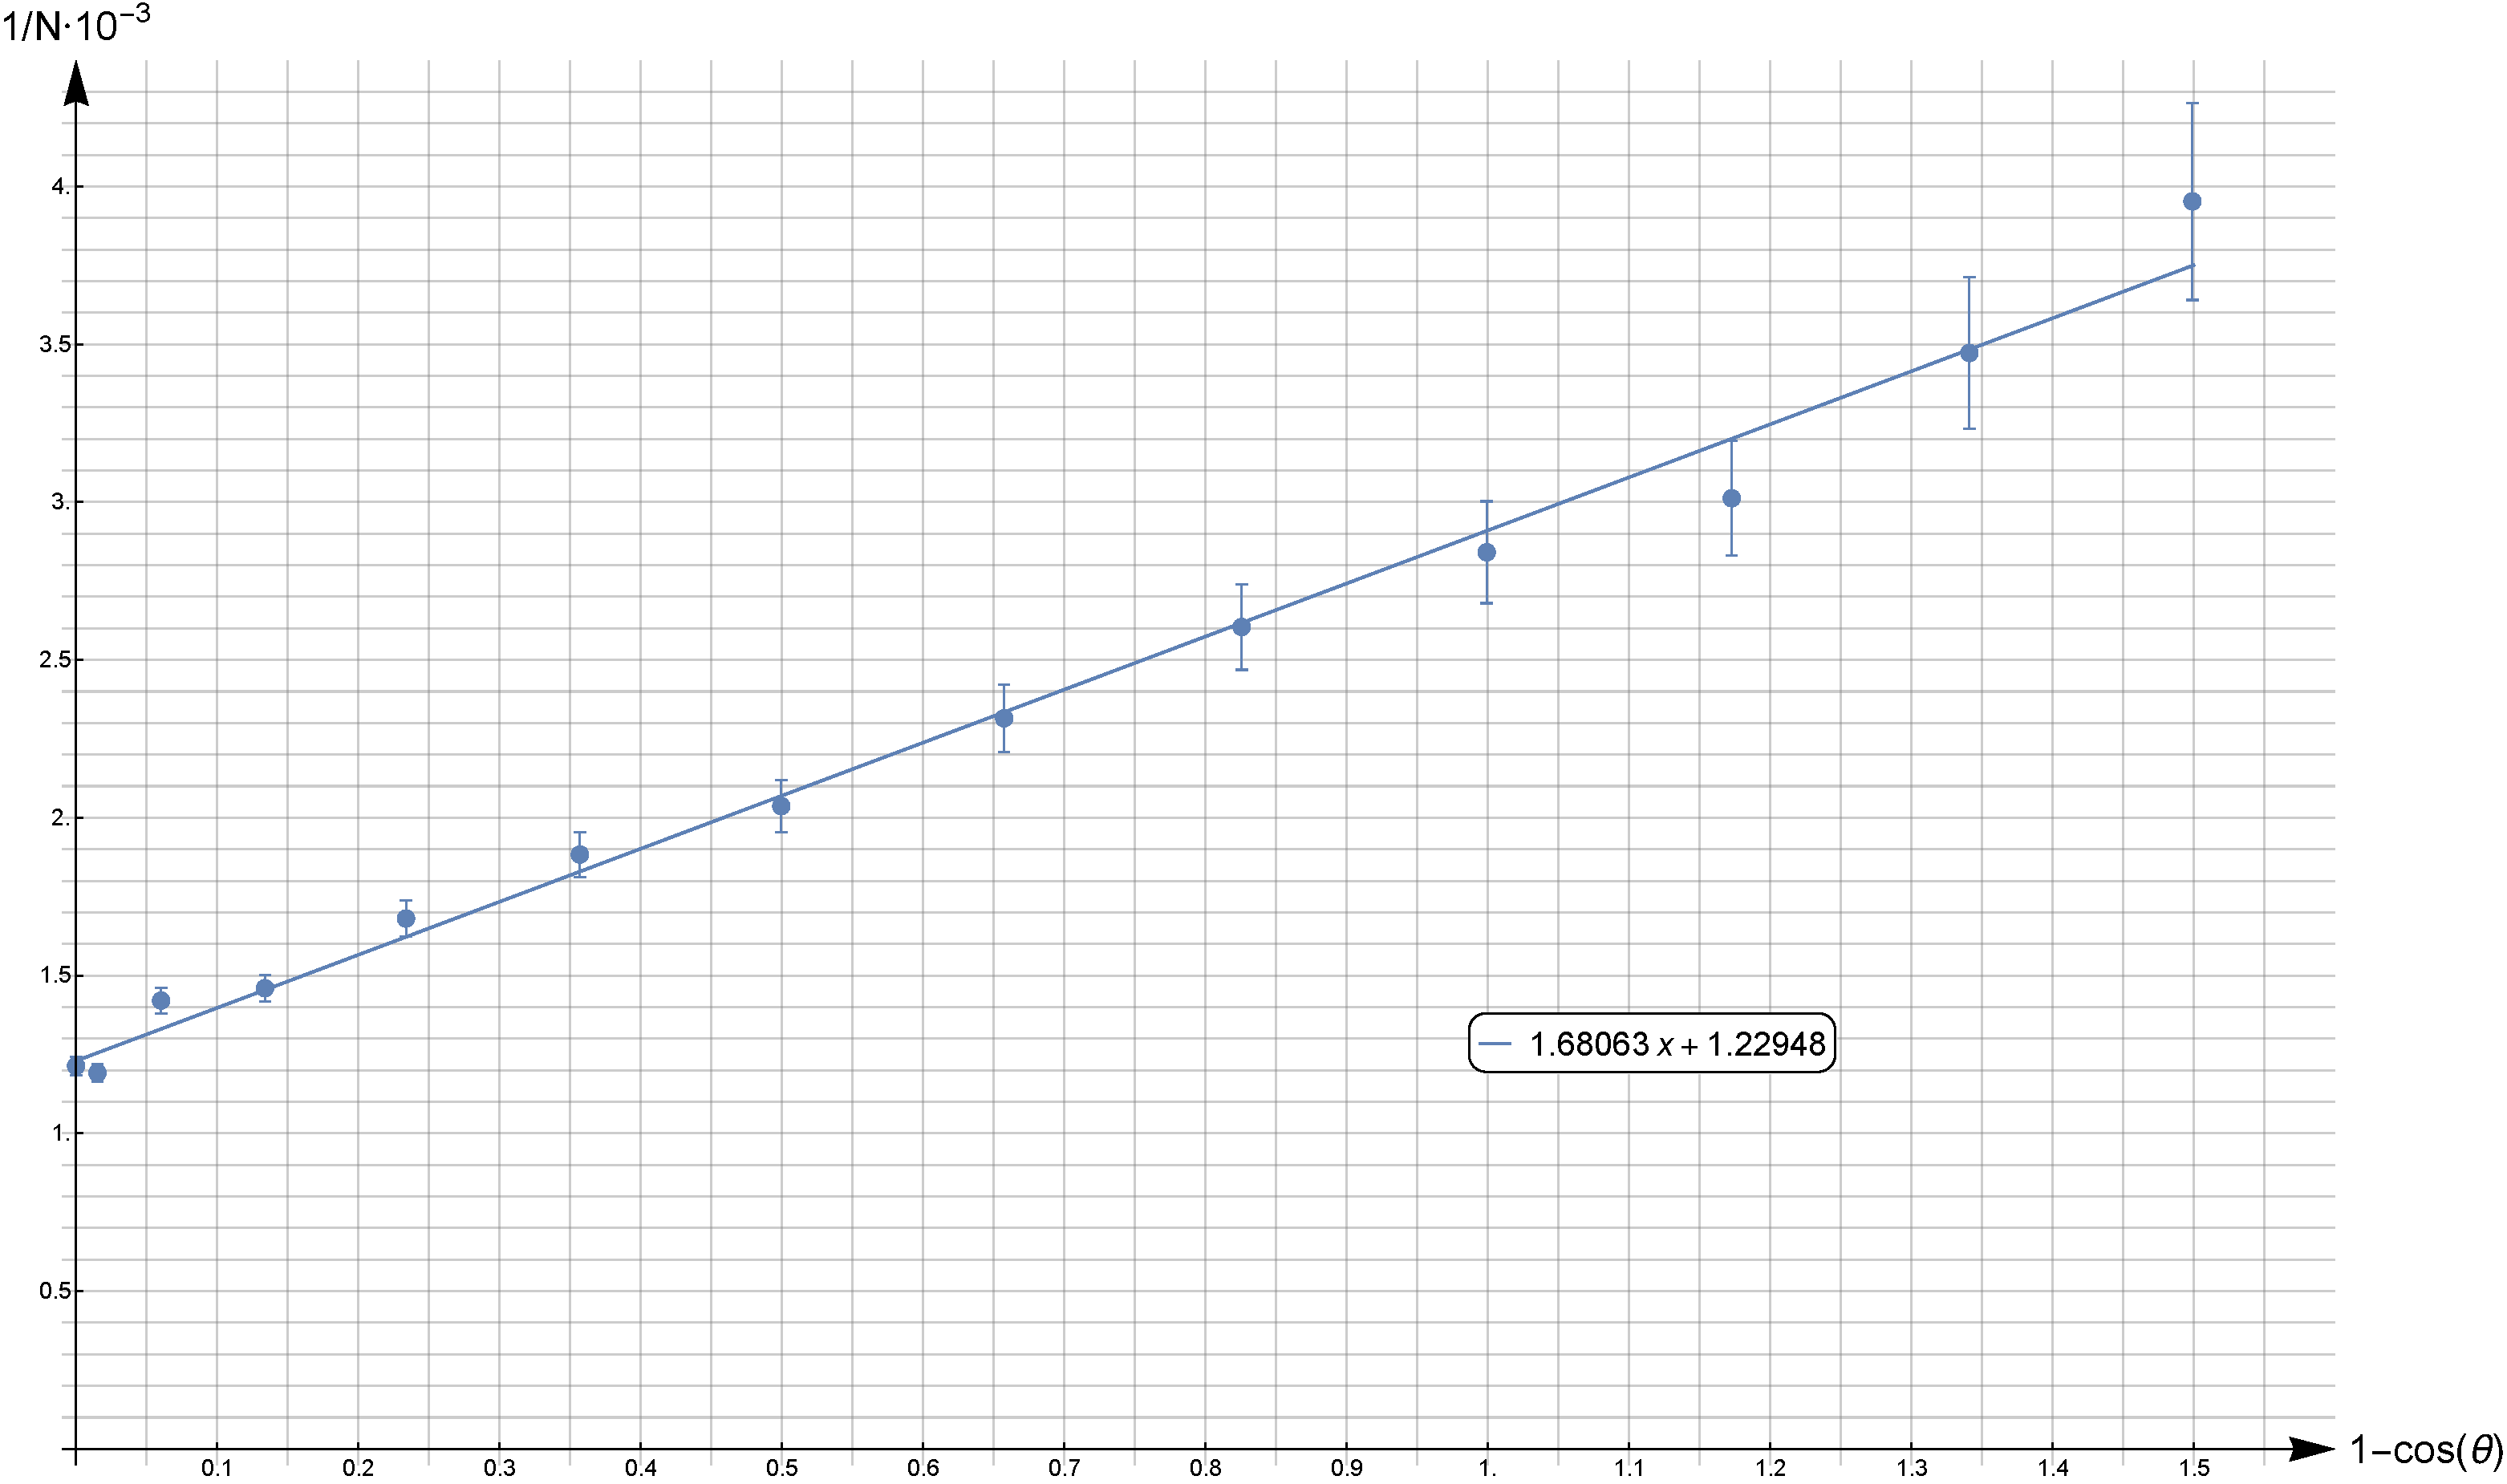
\includegraphics[width=0.8\linewidth]{6}}        
    \end{floatrow}
\end{figure}

Простыми
тригонометрическим преобразованием
уравнения выше можно найти спектр
амплитудно-модулированных колебаний:

\begin{equation}
\begin{aligned}
f(t) &= A_{0} \cos \left(\omega_{0} t\right)+A_{0} m \cos (\Omega t) \cos \left(\omega_{0} t\right) =\\ &= A_{0} \cos \left(\omega_{0} t\right)+\frac{A_{0} m}{2} \cos \left(\omega_{0}+\Omega\right) t+\frac{A_{0} m}{2} \cos \left(\omega_{0}-\Omega\right) t
\end{aligned}
\end{equation}

\section{Оборудование}
\textbf{В работе
используются:} персональный компьютер;
USB-осциллограф АКИП-4107;
функциональный генератор WaveStation
2012; соединительные кабели.

\subsection*{Экспериментальная установка}
\begin{figure}[H]
    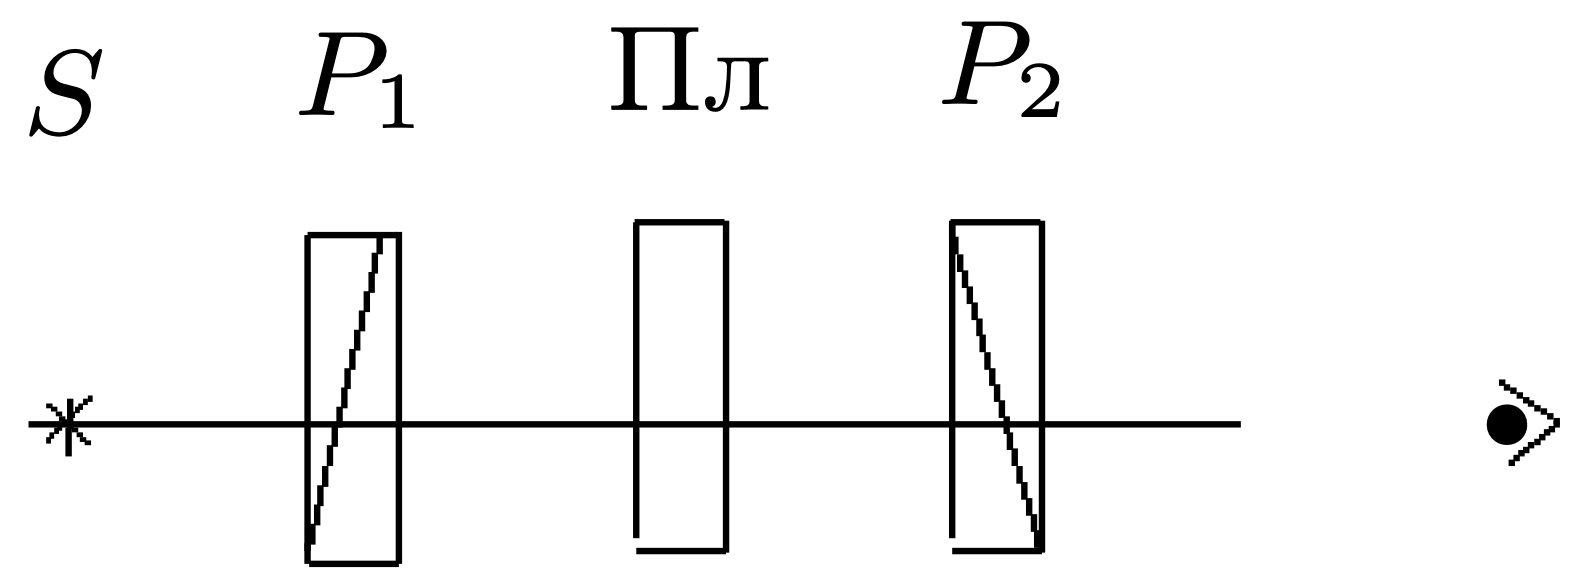
\includegraphics[width=0.725\linewidth]{7} 
    \captionsetup{justification=centering}
    \caption{Схема установки для
    исследования спектра периодических
электрических сигналов различной формы}
\end{figure}
Функциональный генератор WaveStation
2012 позволяет сформировать два
различных электрических сигнала, которые
выводятся на два независимых канала –
<<CH1>> и <<CH2>>. Сигнал с канала
<<CH1>>
подается на вход <<A>>, а сигнал с канала
<<CH2>> – на вход <<B>> USB-осциллографа.
Затем эти сигналы подаются на вход
компьютера через USB-соединение. При
работе USB- осциллографа в режиме
осциллографа, на экране компьютера можно
наблюдать каждый из сигналов в
отдельности, а также их произведение. В
режиме спектроанализатора можно
наблюдать спектры этих сигналов.

\section{Результаты измерений и обработка результатов}
\subsection*{Исследование спектра
периодической последовательности
прямоугольных импульсов}
Установим параметры:
\renewcommand{\arraystretch}{1.1} 
\begin{table}[H]
\begin{tabular}{|c|c|c|c|}
    \hline
    Ampl, \text{В} & Offset, \text{В} &
    Freq ($f_\text{повт}$), \text{кГц} &
    PulWidth ($\tau$), \text{мкс} \\
    \hline
    1 & 0,5 & 1 & 100 \\ \hline 
    
\end{tabular}
\end{table}
Ampl -- разность максимального и
минимального значений сигнала, Offset -
смещение сигнала, Freq - частота
повторения импульсов, PulWidth --
длительность импульса.
    

При увеличении $\tau$ вдвое при
неизменной частоте $f_\text{повт} = 1 \
\text{кГц}$ $\Delta \nu$
уменьшилось в два раза, $\delta \nu$
не изменилось. При увеличении $f_\text{повт}$ вдвое при
неизменном $\tau = 100 \ \text{мкс}$
$\Delta \nu$ не изменилось, а $\delta
\nu$ увеличилось вдвое. (рис. 2)

Проведем измерения зависимости ширины
спектра $\Delta \nu$ от длительности
импульса $\tau$.

\begin{table}[H]
\centering
\begin{tabular}{|c|c|c|c|c|c|c|c|c|c|}
\hline
$\tau, \ \text{мкс}$  & 40 & 60   & 80   & 100 & 120 & 140 & 160 & 180 & 200 \\ \hline
$\Delta \nu, \ \text{кГц}$ & 25 & 17,5 & 12,5 & 10  & 8,5 & 7   & 6   & 5,5 & 5   \\ \hline
\end{tabular}
\captionsetup{justification=centering}
\caption{Зависимость ширины спектра
$\Delta \nu$ от длительности импульса
$\tau$}
\label{tab:first}
\end{table}

По данным в таблице \ref{tab:first}
построим график $\Delta \nu(1/\tau)$ 
\begin{figure}[H]
    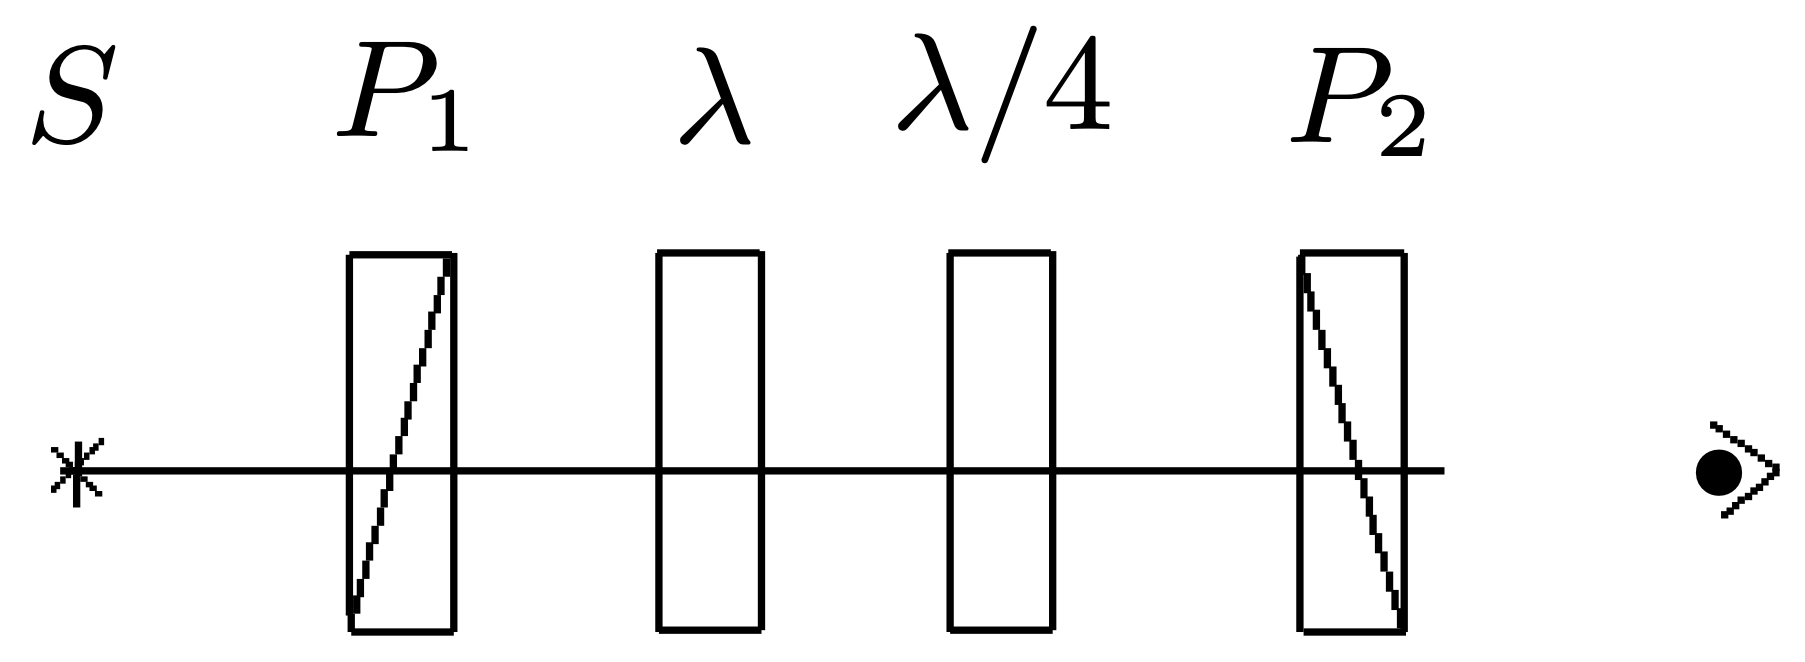
\includegraphics[width=0.8\linewidth]{8} 
    \captionsetup{justification=centering}
    \caption{График зависимости ширины
    спектра $\Delta \nu$ от величины,
обратной к длительности импульса $1/\tau$}
\end{figure}

Измерим частоты и амплитуды спектральных
составляющих сигнала и запишем
результаты в таблицу. № гармоники
численно совпадает с $\nu$, измеренной в
$\text{кГц}$
\renewcommand{\arraystretch}{1.1} 
\renewcommand{\tabcolsep}{1.4mm} 
\begin{table}[H]
\centering
\begin{tabular}{|c|c|c|c|c|c|c|c|c|c|c|}
\hline
$\nu, \ \text{кГц}$ & 1      & 2      & 3      & 4      & 5      & 6      & 7      & 8      & 9      & 10     \\ \hline
$U_a, \text{B}$ & 0,137  & 0,130  &
0,118  & 0,103  & 0,086  & 0,067  &
0,048  & 0,030  & 0,014  & 0,001  \\
\hline \hline
$\nu, \ \text{кГц}$ & 11     & 12     & 13     & 14     & 15     & 16     & 17     & 18     & 19     & 20     \\ \hline
$U_a, \text{B}$ & -0,011 & -0,020 &
-0,027 & -0,030 & -0,030 & -0,026 &
-0,022 & -0,015 & -0,007 & -0,001 \\
\hline \hline
$\nu, \ \text{кГц}$ & 21     & 22     & 23     & 24     & 25     & 26     & 27     & 28     & 29     & 30     \\ \hline
$U_a, \text{B}$ & 0,006  & 0,011  &
0,015  & 0,016  & 0,016  & 0,015  &
0,012  & 0,009  & 0,005  & 0,001  \\
\hline \hline
$\nu, \ \text{кГц}$ & 31     & 32     & 33     & 34     & 35     & 36     & 37     & 38     & 39     & 40     \\ \hline
$U_a, \text{B}$ & -0,004 & -0,008 & -0,011 & -0,012 & -0,013 & -0,012 & -0,010 & -0,007 & -0,004 & 0,000  \\ \hline
\end{tabular}
\captionsetup{justification=centering}
\caption{Частоты и амплитуды
спектральных составляющих сигнала при
$f_\text{повт} = 1 \ \text{кГц}$, $\tau
= 50 \ \text{мкс}$}
\end{table}

\begin{table}[H]
\centering
\begin{tabular}{|c|c|c|c|c|c|c|c|c|c|c|}
\hline
$\nu, \ \text{кГц}$ & 1      & 2      & 3      & 4      & 5      & 6      & 7      & 8      & 9      & 10     \\ \hline
$U_a, \text{B}$ & 0,069  & 0,068  &
0,066  & 0,063  & 0,060  & 0,057  &
0,052  & 0,048  & 0,043  & 0,038  \\
\hline \hline
$\nu, \ \text{кГц}$ & 11     & 12     & 13     & 14     & 15     & 16     & 17     & 18     & 19     & 20     \\ \hline
$U_a, \text{B}$ & 0,033  & 0,029  &
0,024  & 0,019  & 0,016  & 0,012  &
0,009  & 0,006  & 0,004  & 0,001  \\
\hline \hline
$\nu, \ \text{кГц}$ & 21     & 22     & 23     & 24     & 25     & 26     & 27     & 28     & 29     & 30     \\ \hline
$U_a, \text{B}$ & -0,003 & -0,006 &
-0,008 & -0,010 & -0,011 & -0,012 &
-0,013 & -0,013 & -0,014 & -0,014 \\
\hline \hline
$\nu, \ \text{кГц}$ & 31     & 32     & 33     & 34     & 35     & 36     & 37     & 38     & 39     & 40     \\ \hline
$U_a, \text{B}$ & -0,014 & -0,013 & -0,012 & -0,011 & -0,010 & -0,008 & -0,006 & -0,004 & -0,003 & -0,001 \\ \hline
\end{tabular}
\captionsetup{justification=centering}
\caption{Частоты и амплитуды
спектральных составляющих сигнала при
$f_\text{повт} = 1 \ \text{кГц}$, $\tau
= 100 \ \text{мкс}$}
\end{table}

\begin{figure}[H]
    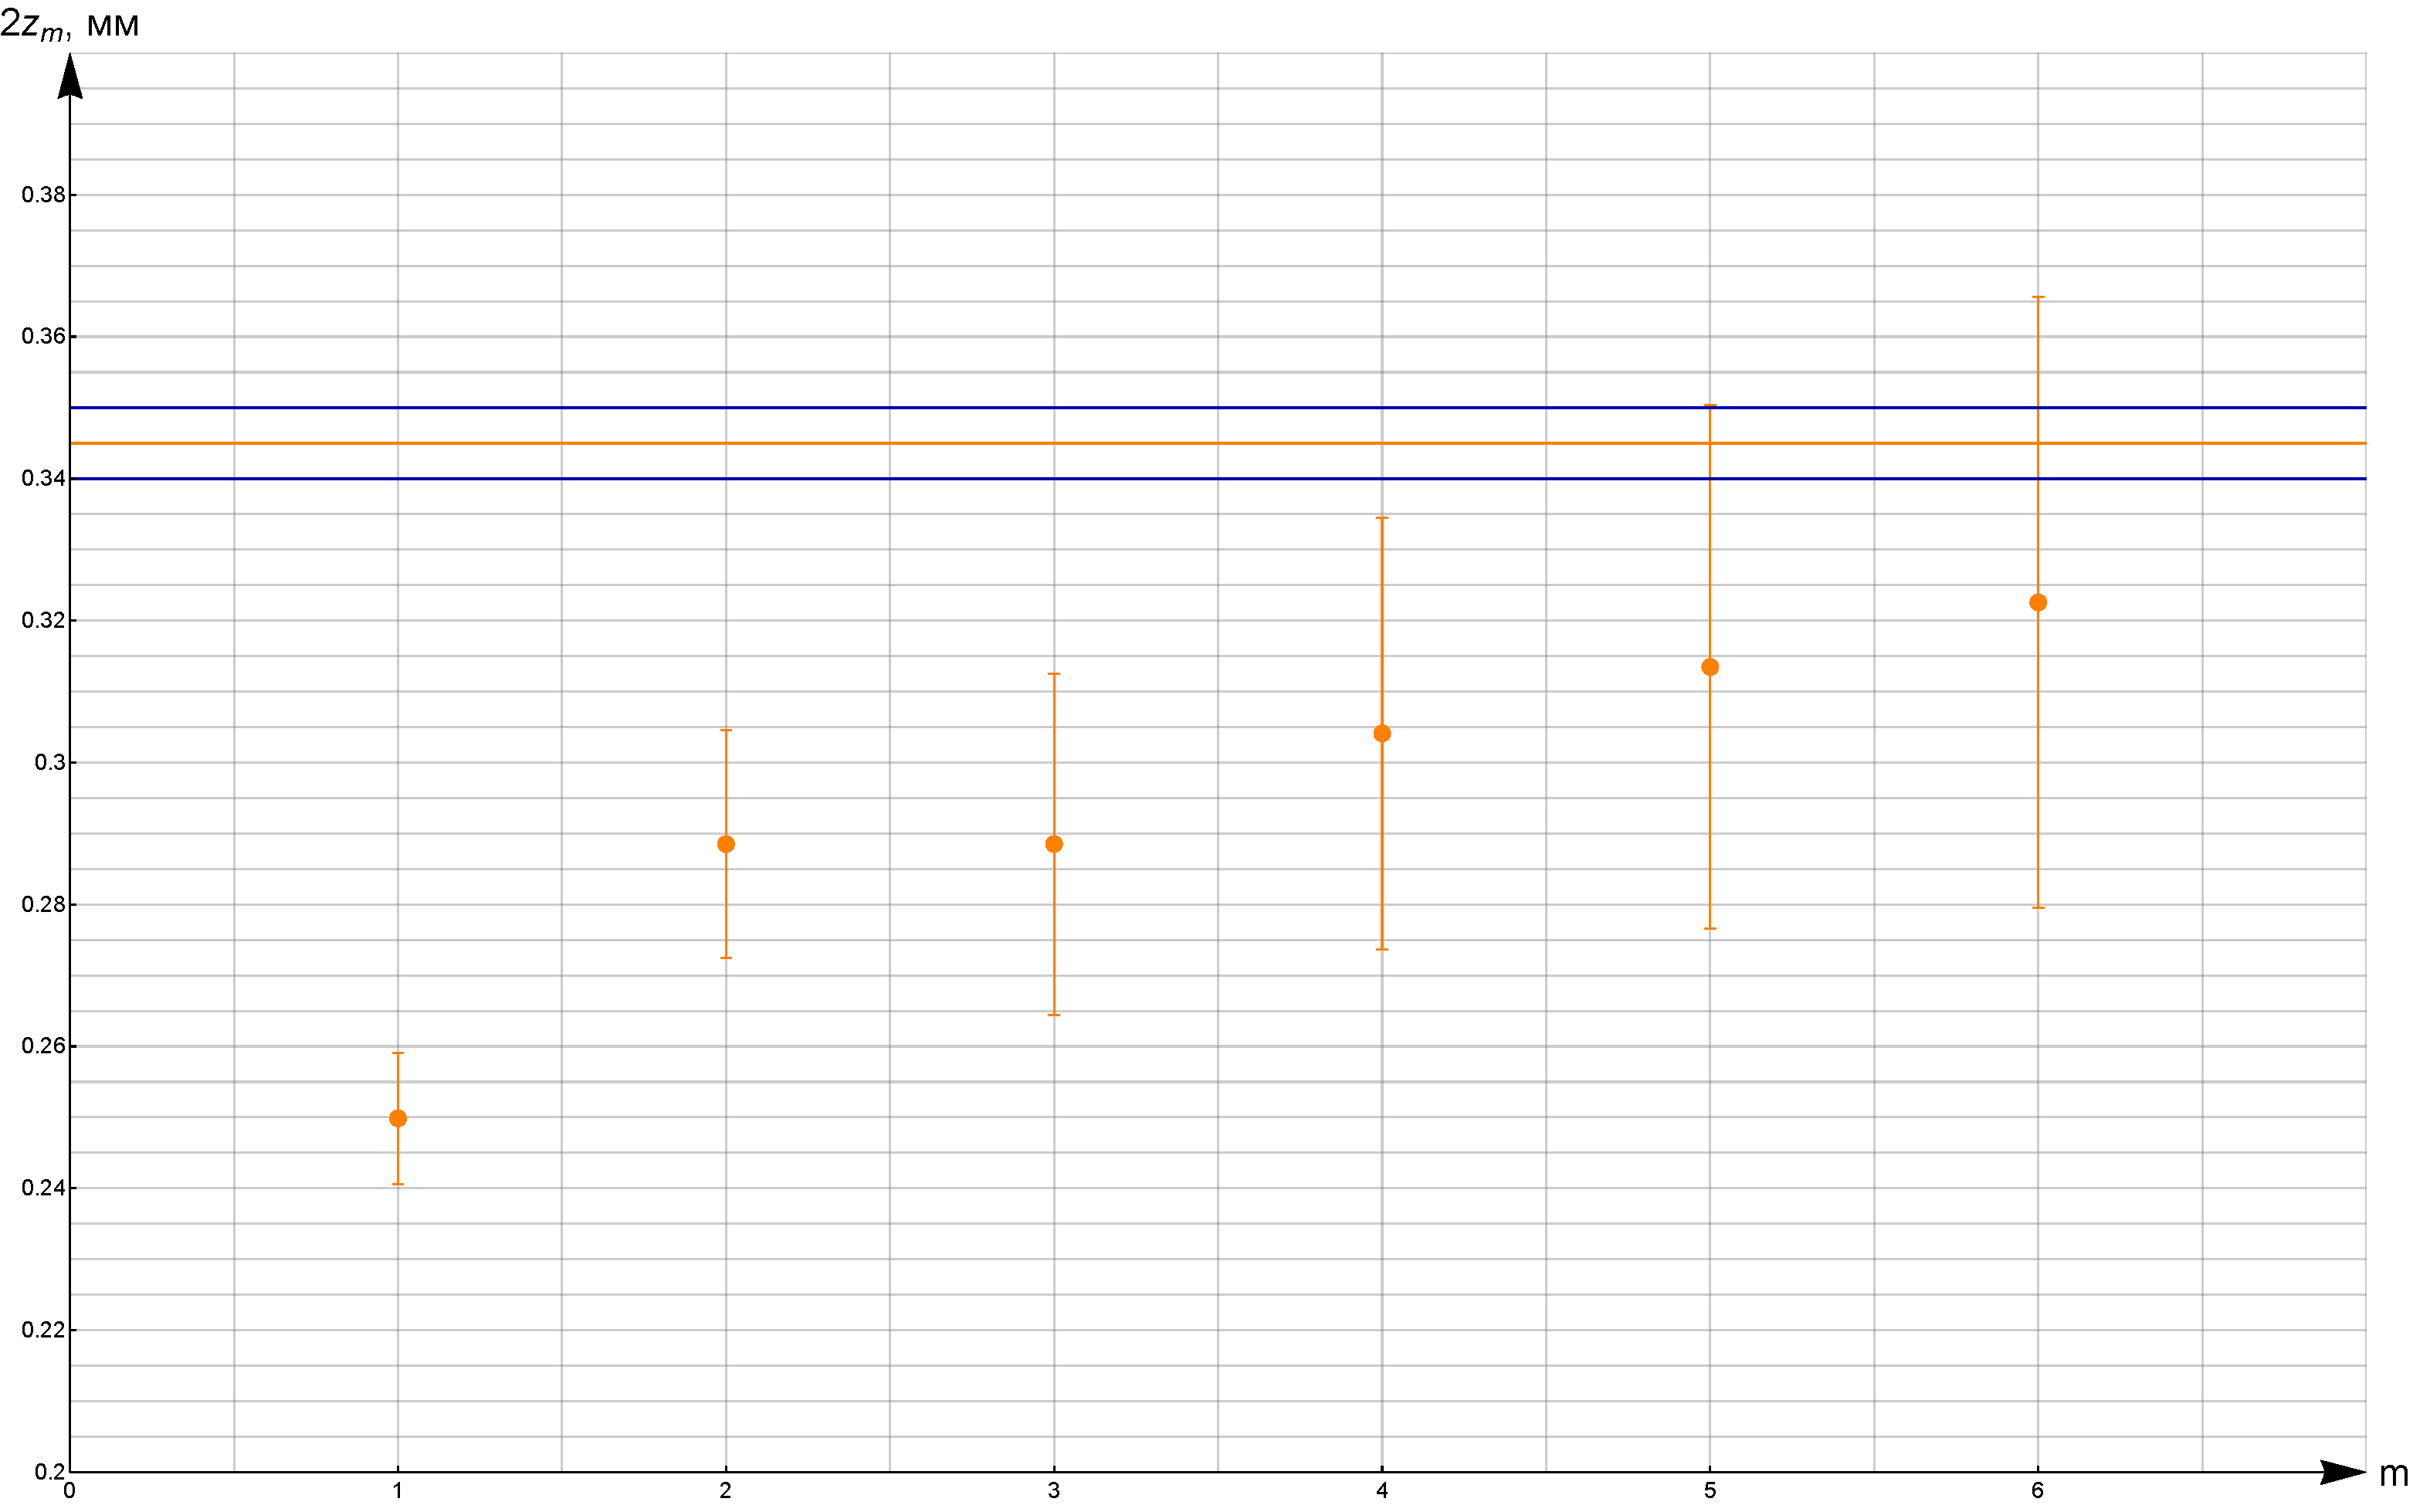
\includegraphics[width=0.95\linewidth]{9} 
    \captionsetup{justification=centering}
    \caption{Спектр периодической
    последовательности прямоугольных
импульсов}
\end{figure}

\subsection*{Исследование спектра
периодической последовательности цугов
гармонических колебаний}

Выставим параметры генератора
\renewcommand{\arraystretch}{1.1} 
\begin{table}[H]
\begin{tabular}{|c|c|c|c|c|c|}
    \hline
     & Сигнал & Ampl, \text{В} & Offset, \text{В} &
    Freq ($f_\text{повт}$), \text{кГц} &
    PulWidth ($\tau$), \text{мкс} \\
    \hline
    CH1 & Pulse & 1 & 0,5 & 1 & 100 \\
    \hline
    CH2 & Sine & 2 & 0 & 25 & \\ \hline
\end{tabular}
\end{table}

При увеличении длительности импульса $\tau$
вдвое $\Delta \omega$ уменьшается в 2
раза, $\omega_0$ и $\delta \omega$ не
изменяются (рис. 4).

Установим длительность импульса $\tau =
100 \ \text{мкс}$. При увеличении частоты
$\nu_0$
на <<CH2>> ($\nu_0 = 10,\ 25,\ 40 \
\text{кГц}$) значения $\omega_0$ равны
соответственно 10, 25, 40
$\text{кГц}$; $\Delta \omega$ и $\delta \omega$ не
изменяются и равны $10 \ \text{кГц}$, $1 \ \text{кГц}$

Установим частоту несущей $\nu_0 = 30 \
\text{кГц}$. Длительность импульса $\tau
= 100 \ \text{мкс}$. Снимем зависимость
расстояния $\delta \omega$ между
соседними спектральными компонентами от 
разных частот повторения импульсов
$f_\text{повт}$

\begin{table}[H]
    \renewcommand{\arraystretch}{1.2} 
    \begin{tabular}{|c|c|c|c|c|c|}
        \hline
        $f_\text{повт}, \ \text{кГц}$ &
        0,52 & 1,02 & 2,03 & 4,02 & 5,01 \\ \hline
        $\delta \omega, \ \text{кГц}$ &
        0,51 & 1,01 & 2,01 & 4,04 & 5,02 \\ \hline
    \end{tabular}
    \captionsetup{justification=centering}
    \caption{Зависимость расстояния
    $\delta \omega$ от разных частот
повторения импульсов}
\end{table}

\begin{figure}[H]
    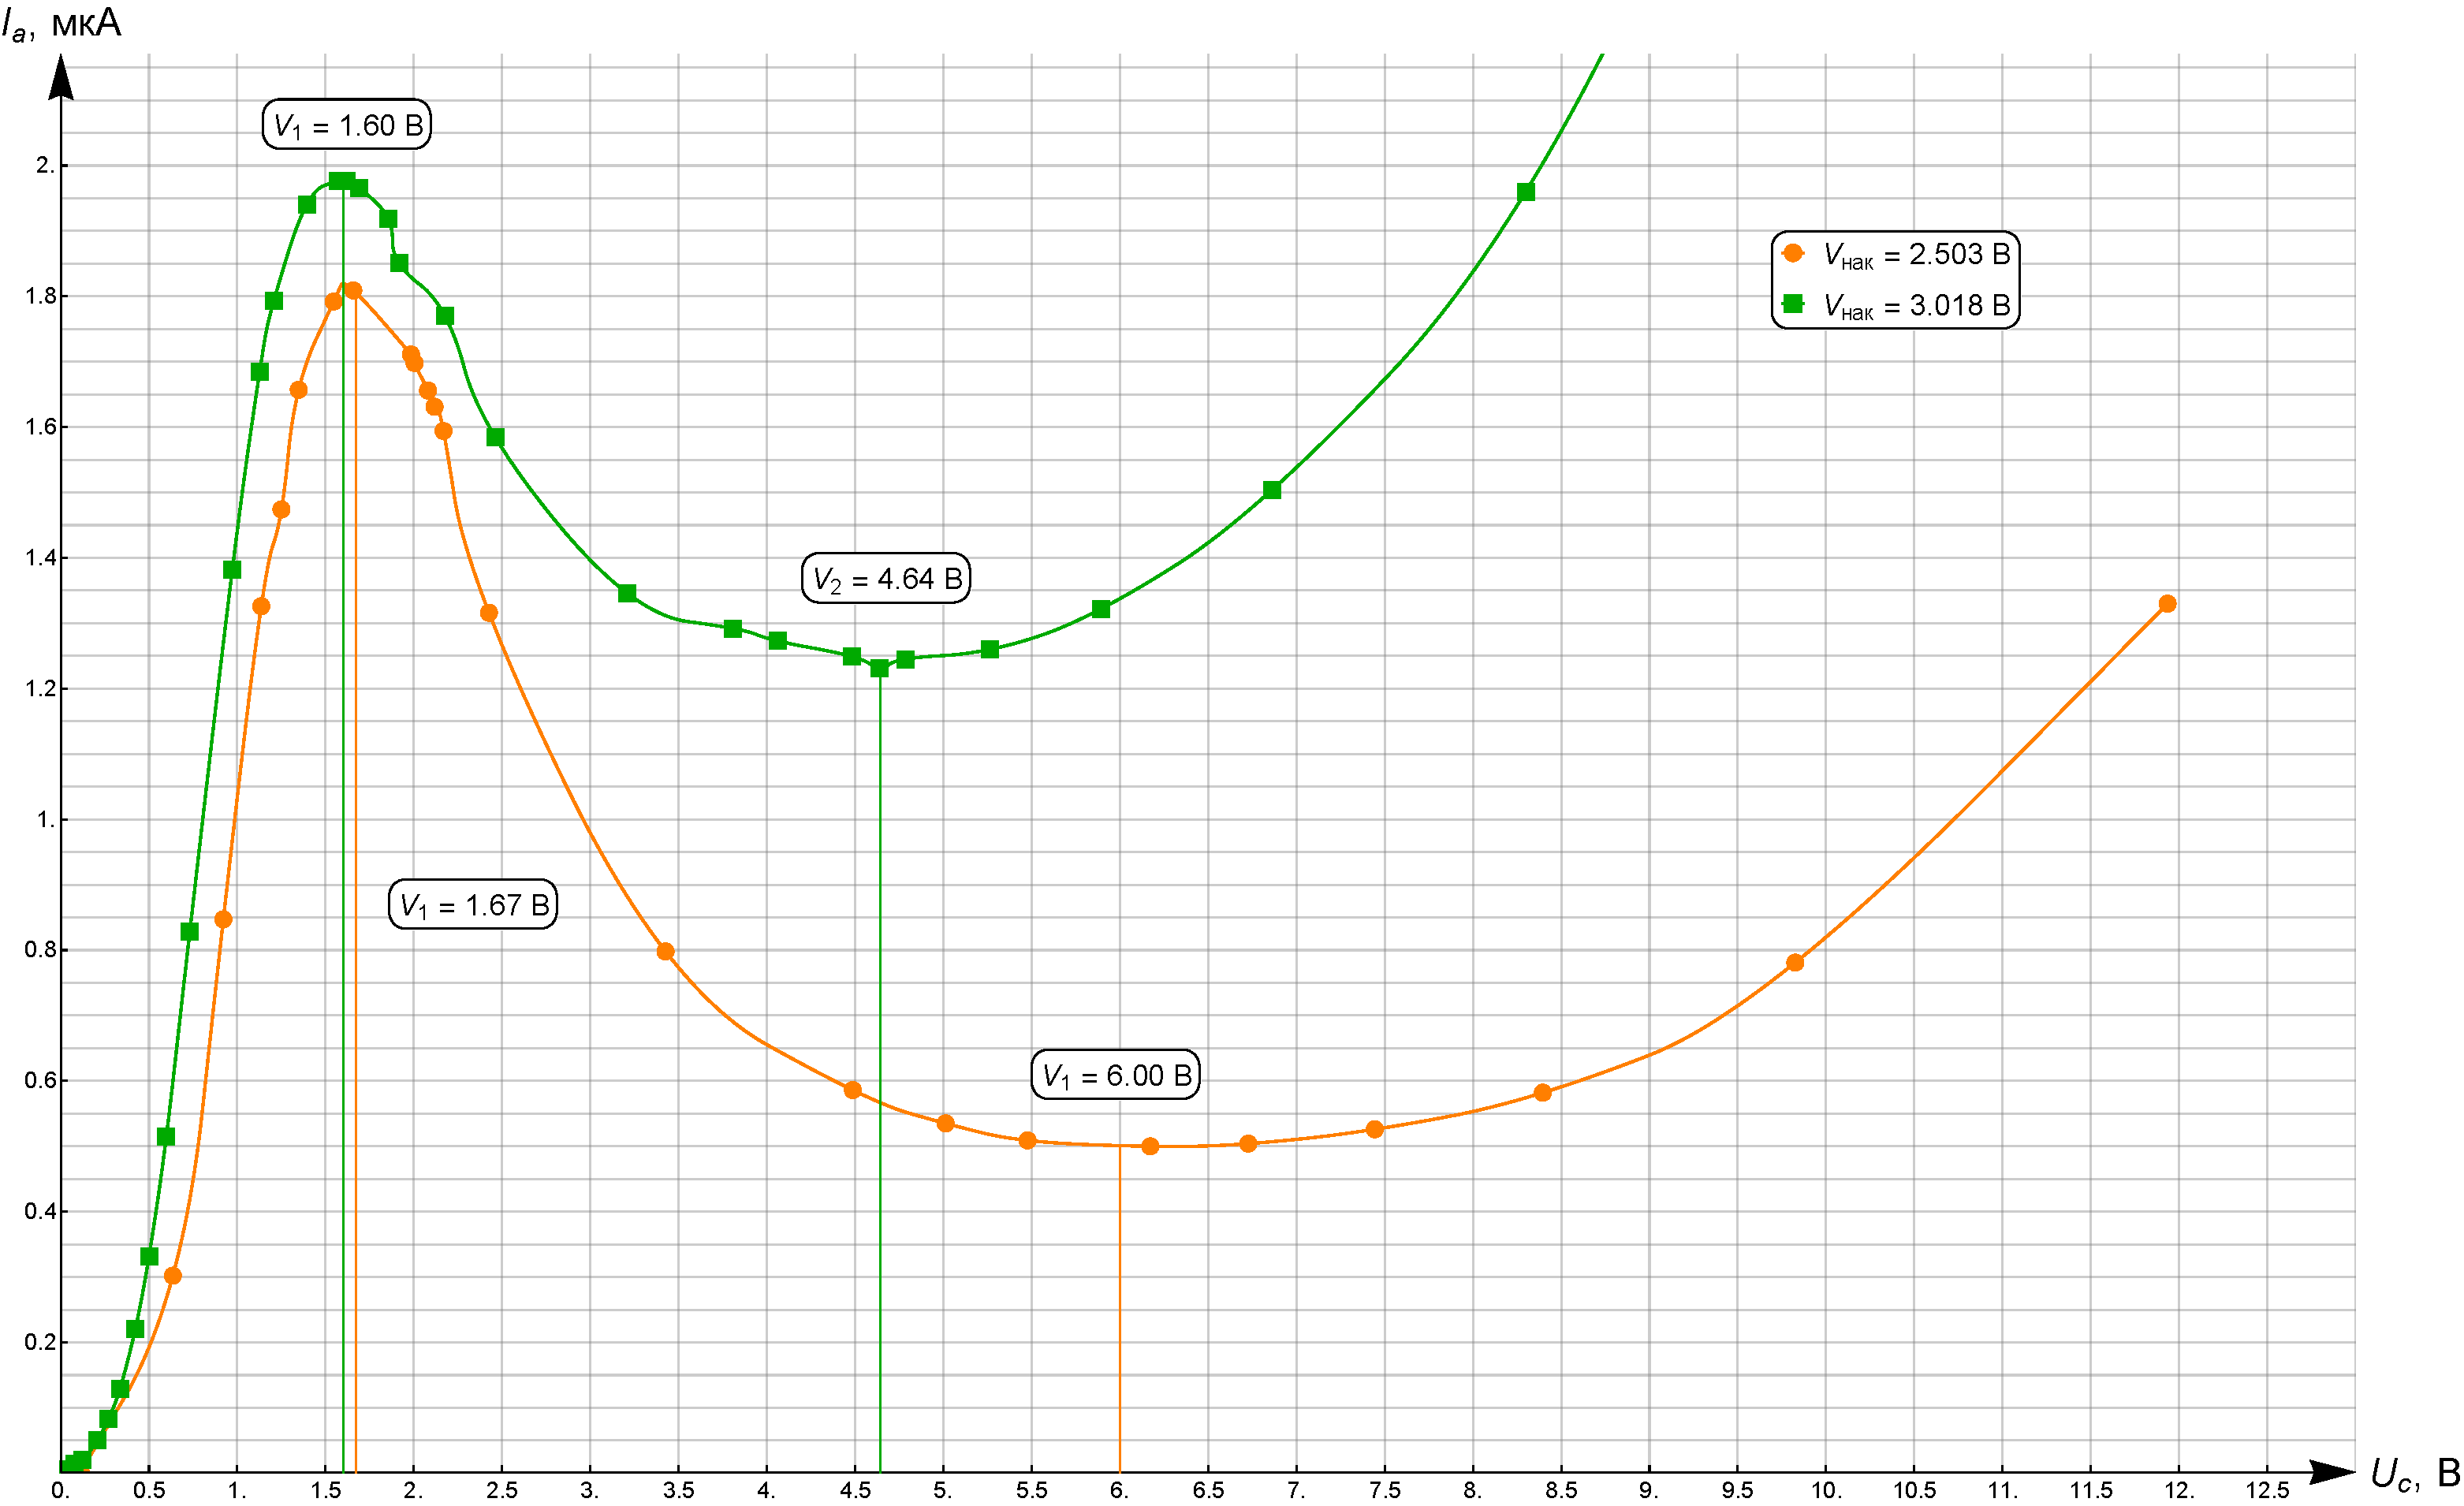
\includegraphics[width=0.9\linewidth]{10} 
    \captionsetup{justification=centering}
    \caption{Зависимость расстояния
    $\delta \omega$ от разных частот
повторения импульсов}
\end{figure}

Установим $\tau = 100 \ \text{мкс}$ и
$f_\text{повт} = 1 \ \text{кГц}$. Снимем
амплитудно-частотную характеристику.
Тоже самое проделаем для импульса с
$\tau = 100 \ \text{мкс}$ и
$f_\text{повт} = 2 \ \text{кГц}$.

\begin{table}[H]
\centering
\begin{tabular}{|c|c|c|c|c|c|c|c|c|c|c|}
\hline
$\nu, \ \text{кГц}$ & 1      & 2      & 3      & 4      & 5      & 6      & 7      & 8      & 9      & 10     \\ \hline
$U_a, \text{мB}$ & 0,160  & 0,280  &
0,382  & 0,458  & 0,486  & 0,468  &
0,412  & 0,324  & 0,210  & 0,038  \\
\hline \hline
$\nu, \ \text{кГц}$ & 11     & 12     & 13     & 14     & 15     & 16     & 17     & 18     & 19     & 20     \\ \hline
$U_a, \text{мB}$ & -0,109 & -0,252 &
-0,377 & -0,469 & -0,531 & -0,532 &
-0,484 & -0,384 & -0,231 & 0,112  \\
\hline \hline
$\nu, \ \text{кГц}$ & 21     & 22     & 23     & 24     & 25     & 26     & 27     & 28     & 29     & 30     \\ \hline
$U_a, \text{мB}$ & 0,431  & 0,911  &
1,385  & 1,825  & 2,209  & 2,353  &
2,688  & 2,934  & 3,112  & 14,330 \\
\hline \hline
$\nu, \ \text{кГц}$ & 31     & 32     & 33     & 34     & 35     & 36     & 37     & 38     & 39     & 40     \\ \hline
$U_a, \text{мB}$ & 3,069  & 2,846  & 2,549  & 2,197  & 1,825  & 1,414  & 1,015  & 0,653  & 0,350  & 0,114  \\ \hline
\end{tabular}
\captionsetup{justification=centering}
\caption{Амплитудно-частотная
характеристика спектра цугов при $\tau = 100 \
\text{мкс}$ и $f_\text{повт} = 1 \
\text{кГц}$}
\end{table}

\begin{table}[H]
\centering
\begin{tabular}{|c|c|c|c|c|c|c|c|c|c|c|}
\hline
$\nu, \ \text{кГц}$ & 2     & 4     & 6     & 8     & 10     & 12     & 14     & 16     & 18     & 20    \\ \hline
$U_a, \text{мB}$  & 0,543 & 0,856 & 0,721
& 0,527 & 0,038  & -0,773 & -1,203 &
-1,307 & -0,97 & 0,030 \\ \hline \hline
$\nu, \ \text{кГц}$ & 22    & 24    & 26    & 28    & 30     & 32     & 34     & 36     & 38     & 40    \\ \hline
$U_a, \text{мB}$  & 1,923 & 3,750 & 5,044 & 5,999 & 17,545 & 5,648  & 4,337  & 2,688  & 1,158  & 0,035 \\ \hline
\end{tabular}
\captionsetup{justification=centering}
\caption{Амплитудно-частотная
характеристика спектра цугов при $\tau = 100 \
\text{мкс}$ и $f_\text{повт} = 2 \
\text{кГц}$}
\end{table}

\begin{figure}[H]
    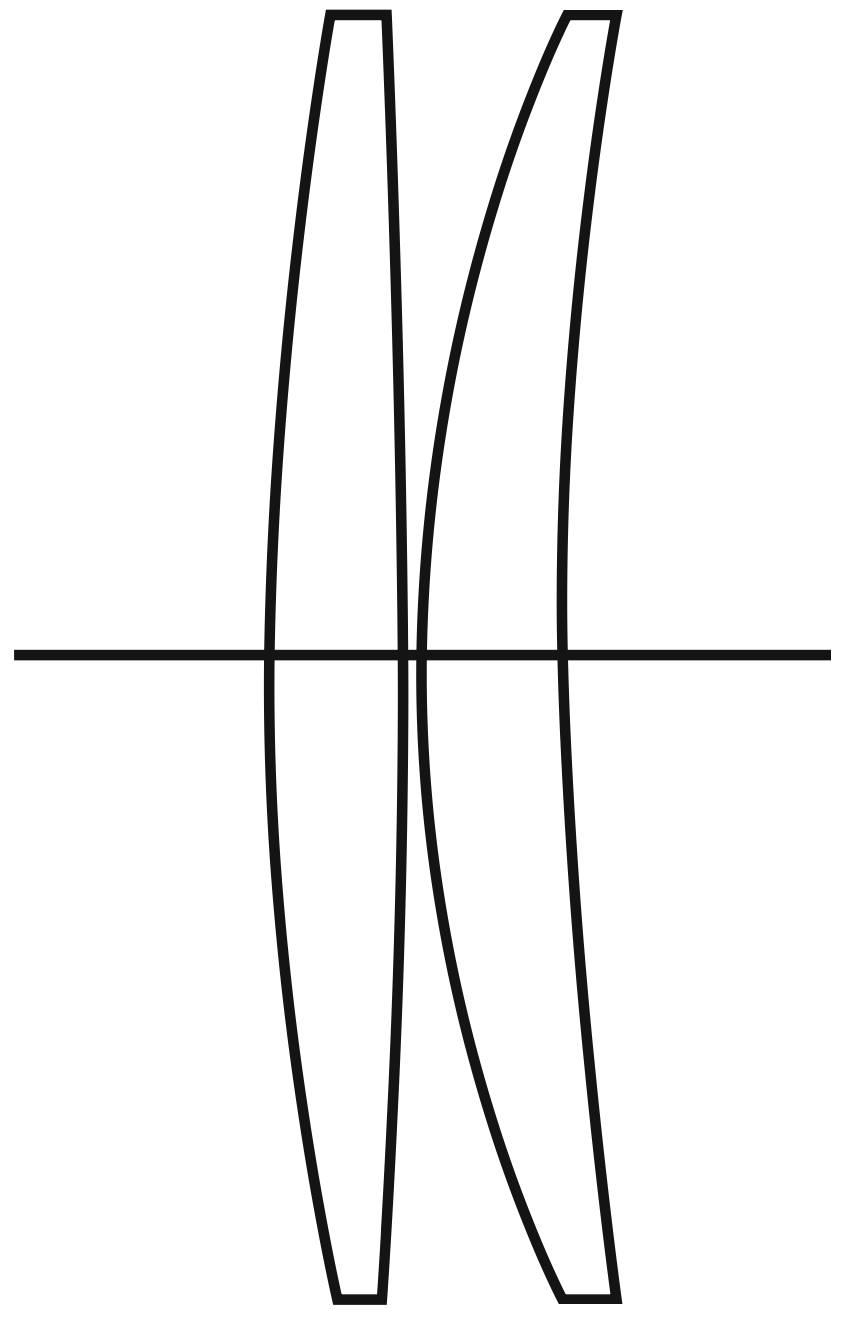
\includegraphics[width=\linewidth]{11} 
    \captionsetup{justification=centering}
    \caption{Амплитудно-частотная
    характеристика спектра цугов при
$\tau = 100 \ \text{мкс}$ и
$f_\text{повт} = 1, 2 \ \text{кГц}$}
\end{figure}


\subsection*{Исследование спектра
гармонических сигналов, модулированных
по амплитуде}
Выставим параметры на генераторе:

\renewcommand{\arraystretch}{1.1} 
\begin{table}[H]
\begin{tabular}{|c|c|c|c|c|}
    \hline
     & Сигнал & Ampl, \text{В} & Offset, \text{В} &
    Freq ($f_\text{повт}$), \text{кГц}
    \\
    \hline
    CH1 & Sine & 0,2 & 1 & 1  \\
    \hline
    CH2 & Sine & 1 & 0 & 25  \\ \hline
\end{tabular}
\end{table}
Меняя двойную амплитуду сигнала канала
<<CH1>> от $0,2$ до $2 \ \text{В}$
измеряем максимальную $A_{max}$ и
минимальную $A_{min}$ амплитуды сигналов
модулированного колебания и амплитуды
спектральных компонент. 

\begin{table}[H]
\centering
\begin{tabular}{|c|c|c|c|c|c|c|}
\hline
$Ampl, \ \text{В}$ & $A_{max}, \
\text{В}$  & $A_{min}, \ \text{В}$  &
$A_{\text{осн}}, \ \text{B}$   &
$A_\text{бок}, \ \text{В}$  &
$A_{\text{бок}}/A_{\text{осн}}$ & $m$    \\ \hline
0,2 & 0,547 & 0,439 & 0,322 & 0,016 & 0,05     & 0,11 \\ \hline
0,4 & 0,600 & 0,399 & 0,320 & 0,032 & 0,10     & 0,20 \\ \hline
0,6 & 0,643 & 0,340 & 0,320 & 0,048 & 0,15     & 0,31 \\ \hline
0,8 & 0,678 & 0,311 & 0,324 & 0,056 & 0,17     & 0,37 \\ \hline
1,0 & 0,749 & 0,250 & 0,330 & 0,081 & 0,25     & 0,50 \\ \hline
1,2 & 0,769 & 0,202 & 0,333 & 0,095 & 0,28     & 0,58 \\ \hline
1,6 & 0,888 & 0,092 & 0,320 & 0,129 & 0,40     & 0,81 \\ \hline
2,0 & 0,989 & 0,010 & 0,318 & 0,164 & 0,52     & 0,98 \\ \hline
\end{tabular}
\captionsetup{justification=centering}
\caption{Максимальная амплитуда
$A_{max}$, минимальная амплитуда
$A_{min}$, амплитуды спектральных
компонент $A_\text{осн}$,
$A_\text{бок}$ и глубина модуляции $m$}
\end{table}

По полученным данным построим график
зависимости отношения
$A_\text{бок}/A_\text{осн}$ от глубины
модуляции $m$

\begin{figure}[H]
    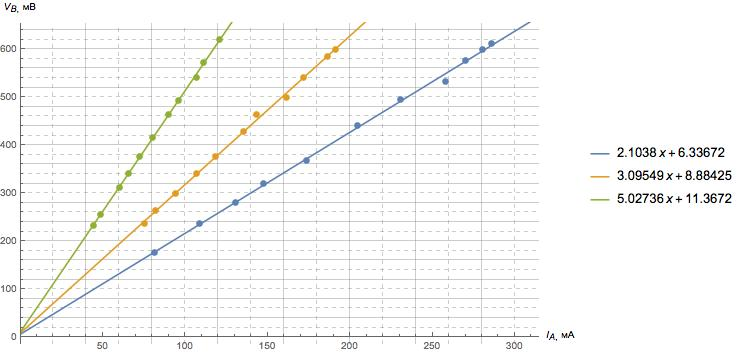
\includegraphics[width=0.8\linewidth]{12} 
    \captionsetup{justification=centering}
    \caption{График
зависимости отношения
$A_\text{бок}/A_\text{осн}$ от глубины
модуляции $m$
}
\end{figure}

При 100\% глубине модуляции ($A_{min} =
0$) при увеличении частоты модуляции
$f_\text{мод}$ в 2 раза ширина спектра
уменьшается в два раза.

\section{Обсуждение результатов и выводы}
Было проведено исследование спектра
периодической последовательности
прямоугольных импульсов (рис. 9) и периодической
последовательности цугов гармонических
колебаний (pис. 11). Уравнение огибающей
совпало с теоретическими расчетами
(рис. 2, формула (6); рис. 4, формула
(7)).

Исследованы
зависимости амплитудно-частотных
характеристик этих спектров от частоты
повторения импульсов $f_\text{повт}$
и их длительности $\tau$. (рис. 8; рис.
10). Было проверено выполнение
соотношения неопределенности (5).
\begin{align*}
    k_1 &= 1,01 \pm 0,01 \ (\text{из
    графика на рис. 8)} \\
    k_2 &= 1,00 \pm 0,01 \ (\text{из
    графика на рис. 10})
\end{align*}
С
хорошей точностью соотношение
выполняется. 

По рис.9 и рис. 11 можно провести
сравнение спектра периодической
последовательности прямоугольных
импульсов и спектра периодической
последовательности цугов гармонических
колебаний при одинаковых $f_\text{повт}$
и $\tau$. Спектры отличаются сдвигом на
несущую частоту.

Исследованы спектры
амплитудно-модулированных гармонических
сигналов в зависимости от частоты
модуляции. Был построен график
зависимости отношения
$A_\text{бок}/A_\text{осн}$ от глубины
модуляции $m$ (рис. 12). Коэффициент
угла наклона графика:
\[
    k_3 = 0,50 \pm 0,01 \ (\text{из графика на
    рис. 12})
\]
Полученное значение совпадает с теоретическим 
(рис. 6, формула (9)).

\end{document}
